\documentclass{article}

% Workshop, double-blind review track at submission; accepted, now camera-ready
% (`final` added per NeurIPS 2026 formatting instructions).
% AgenticLS @ NeurIPS 2026 CFP confirms double-blind review.
\usepackage[dblblindworkshop, final]{neurips_2026}
\workshoptitle{Agentic AI for Biological Discovery: Toward Closed-Loop Life-Science Intelligence}

\usepackage[utf8]{inputenc}
\usepackage[T1]{fontenc}
\usepackage{hyperref}
\usepackage{url}
\usepackage{booktabs}
\usepackage{amsfonts}
\usepackage{amsmath}
\usepackage{nicefrac}
\usepackage{microtype}
\usepackage{xcolor}
\usepackage{longtable}
\usepackage{array}
\usepackage{tikz}
\usepackage{pgfplots}
\pgfplotsset{compat=1.18}
\usepackage{placeins}
\usepackage{float}
\usetikzlibrary{positioning}
\hypersetup{colorlinks=true, linkcolor=black, citecolor=black, urlcolor=black}

\title{From Model Scores to Defensible Agent Decisions: Decision Contracts for Molecular Generation and Docking}

\author{%
  Tuan Cao, Hai Luong, Tuan Dinh \\
  Life AI \\
  \texttt{tuan@lifeai.io, hai.luong@lifeai.io, tuan.dinh@lifeai.io}
}

\begin{document}

\maketitle

\begin{abstract}
Computational drug-discovery pipelines chain generation, ligand preparation, docking, and ranking, but components are usually benchmarked in isolation and preprocessing is often treated as deterministic. We introduce \textbf{DecisionBench-DD v1.0}, a frozen, auditable decision-contract methodology that scores tools by end-to-end candidate yield under task-specific gates, and extend that contract to the LLM agents that increasingly interpret such results. In an ambroxol-conditioned GCase/\textit{GBA1} case study, 66/300 GenMol and 3/300 MolMIM outputs passed chemical qualification (configuration--contract fit, not generator superiority). A contract-aware purchasable-catalogue retrieval policy instead returned 258/300 qualifiers after searching 9.32 million unique molecules, only 804 of which fell in the required seed-similarity band---a configured acquisition-policy comparison, not a symmetric algorithm or compute comparison (Appendix~J). In redocking, Top-1 was unresolved (3/14 vs.\ 2/14), but GNINA recovered more near-native poses within five predictions (8/14 vs.\ 2/14) and produced more geometry-valid poses. Fresh embedding changed 18/69 candidate-screen labels and 3/14 redocking verdicts under a fixed seed, and a property-matched decoy comparison gave an inconclusive risk ratio of 1.46 (95\% CI 0.96--2.12); the 16 frozen candidates are an auditable prioritization set, not validated hits. We then tested whether the same framework's \textbf{evidence-semantics} rules change how an LLM agent interprets this evidence: across three prompting conditions (free-form, prose guidance, explicit numbered contract) replicated 50 times (weaker model) and 5 times (stronger model), nine of ten items were answered correctly in every run. The exception---overturning a null primary endpoint with an attractive secondary one---showed the weaker model's violation rate fall from 64\% (free-form) to 34\% (prose; $p=0.005$) to 28\% (contract; not significant vs.\ prose, $p=0.67$), while the stronger model was correct in all 15 runs but only the contract condition left a rule-cited audit trail: stating the rules at all helps most; formalizing them into a contract adds auditability without a further, resolved accuracy gain. Decision contracts should be frozen to compare tools honestly and to constrain the agents that increasingly sit between pipeline outputs and advancement decisions, while conformer preparation should be treated as an experimental factor and structural proxies calibrated before compounds advance.
\end{abstract}

\section{Introduction}

AI-enabled molecular-design tools are typically evaluated in isolation: generators by validity, uniqueness, diversity, or goal scores, and docking systems by pose RMSD or confidence [1--6]. An operational drug-discovery question is narrower and more consequential: \textbf{under a fixed budget and a specified molecular objective, which tool produces more candidates that survive the next decision?} Attractive component-level metrics can be misaligned with this task: high diversity aids exploration but can conflict with a seed-proximity constraint, and permissive proxies can acquire biological interpretations they were never validated for. This question is no longer only a matter of human review: LLM-based agents increasingly read pipeline outputs and recommend or execute the next step in a discovery workflow [19,20], and such an agent inherits whatever interpretive discipline governs its task, making that discipline itself worth evaluating.

We address this gap with \textbf{DecisionBench-DD v1.0}, organized around four principles: (1)~\textbf{freeze the decision contract}---gates and advancement rules are fixed before results are inspected; (2)~\textbf{compare like with like}---tools receive equivalent task information, with asymmetries made explicit; (3)~\textbf{measure decision yield}---performance propagates through the funnel using the requested count as denominator; and (4)~\textbf{audit transfer and proxy validity}---sensitivity analyses stay subordinate to the frozen primary analysis, and a proxy is not promoted to a biological claim without independent controls.

We instantiate this framework using ambroxol-conditioned analogue generation for GCase, encoded by \textit{GBA1}. Ambroxol is a marketed mucolytic reported to act as a pH-dependent mixed inhibitor and pharmacological chaperone of GCase [7,8], relevant to Gaucher disease and \textit{GBA1}-associated Parkinson's disease, offering resolved structures, a known seed, and a meaningful but difficult neutral-versus-acidic receptor-state question.

Our contributions are: (1) an auditable, equal-budget generator-to-candidate funnel (GenMol [9] vs.\ MolMIM [10]) that evaluates configuration--contract fit rather than universal model superiority; (2) a supporting redocking audit (GNINA [4] vs.\ DiffDock-L [5,6]) that feeds the candidate-screen structural proxy and separates Top-1 ranking, five-pose recovery, geometry validity, and receptor-cropping conditions, disclosed as carrying a box-size asymmetry (\S4.2) rather than standing as an independent tool-superiority claim; (3) property-matched background calibration and fresh-embedding audits showing that conformer preparation can alter both benchmark verdicts and compound-advancement decisions; (4) a frozen 16-candidate prioritization set coupled to an explicit experimental calibration plan; (5) a purchasable-catalogue retrieval baseline showing the bottleneck is finding a seed-similar purchasable molecule at all, not clearing downstream gates once found (\S3.1, Appendix~J); and (6) a replicated probe (2 model tiers $\times$ 3 prompting conditions, 50 Haiku and 5 Sonnet runs per condition) of whether the same contract's evidence-semantics rules change an LLM agent's own interpretation of these results, comparing a free-form baseline against prose guidance and an explicit, rule-cited contract representation of those same rules (\S2.4, \S3.6).

\begin{figure}[t]
\centering
\begin{minipage}{0.50\linewidth}
\centering
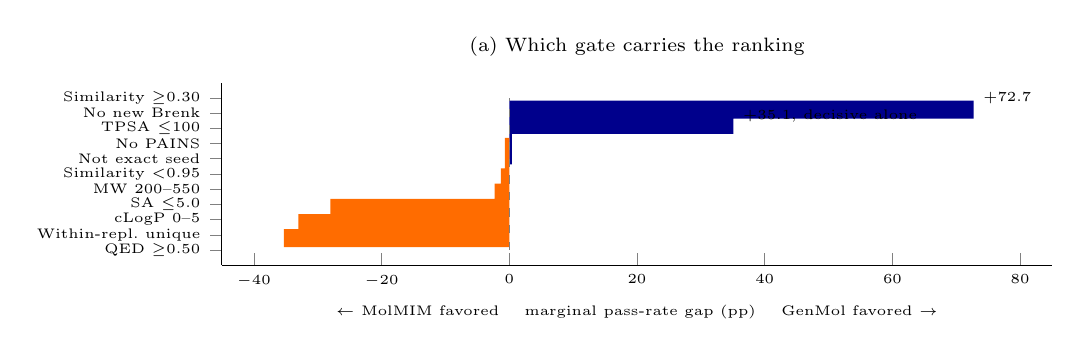
\begin{tikzpicture}
\begin{axis}[
    width=\linewidth, height=3.9cm,
    xbar, bar width=6.5pt,
    xmin=-45, xmax=85,
    xlabel={$\leftarrow$ MolMIM favored \quad marginal pass-rate gap (pp) \quad GenMol favored $\rightarrow$},
    xlabel style={font=\tiny},
    symbolic y coords={QED $\geq$0.50,Within-repl.\ unique,cLogP 0--5,SA $\leq$5.0,MW 200--550,Similarity $<$0.95,Not exact seed,No PAINS,TPSA $\leq$100,No new Brenk,Similarity $\geq$0.30},
    ytick={QED $\geq$0.50,Within-repl.\ unique,cLogP 0--5,SA $\leq$5.0,MW 200--550,Similarity $<$0.95,Not exact seed,No PAINS,TPSA $\leq$100,No new Brenk,Similarity $\geq$0.30},
    y tick label style={font=\tiny},
    tick label style={font=\tiny},
    axis lines*=left,
    title={\scriptsize (a) Which gate carries the ranking},
    clip=false,
]
\addplot[draw=none, fill=blue!55!black] coordinates {
 (72.7,Similarity $\geq$0.30) (35.1,No new Brenk) (0.4,No PAINS) (0.4,TPSA $\leq$100)
};
\addplot[draw=none, fill=orange!85!red] coordinates {
 (-0.7,Not exact seed) (-0.7,Similarity $<$0.95) (-1.3,MW 200--550) (-2.3,SA $\leq$5.0) (-28.0,cLogP 0--5) (-33.0,Within-repl.\ unique) (-35.3,QED $\geq$0.50)
};
\node[anchor=west, font=\tiny] at (axis cs:72.7,Similarity $\geq$0.30) {+72.7};
\node[anchor=west, font=\tiny, yshift=-1pt] at (axis cs:35.1,No new Brenk) {+35.1, decisive alone};
\draw[dashed, black!50] (axis cs:0,QED $\geq$0.50) -- (axis cs:0,Similarity $\geq$0.30);
\end{axis}
\end{tikzpicture}
\end{minipage}
\hfill
\begin{minipage}{0.46\linewidth}
\centering
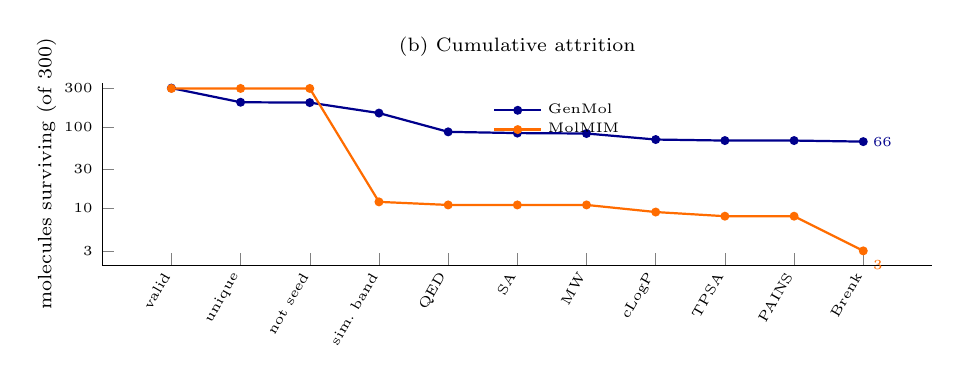
\begin{tikzpicture}
\begin{axis}[
    width=\linewidth, height=3.9cm,
    ymode=log,
    ymin=2, ymax=350,
    ytick={3,10,30,100,300},
    yticklabels={3,10,30,100,300},
    ylabel={molecules surviving (of 300)},
    ylabel style={font=\scriptsize, yshift=-4pt},
    symbolic x coords={valid,unique,not seed,sim.\ band,QED,SA,MW,cLogP,TPSA,PAINS,Brenk},
    xtick={valid,unique,not seed,sim.\ band,QED,SA,MW,cLogP,TPSA,PAINS,Brenk},
    x tick label style={rotate=60, anchor=east, font=\tiny},
    tick label style={font=\tiny},
    axis lines*=left,
    title={\scriptsize (b) Cumulative attrition},
    legend style={font=\tiny, at={(0.55,0.95)}, anchor=north, draw=none, fill=none, row sep=-2pt},
    legend cell align=left,
    clip=false,
]
\addplot[blue!55!black, thick, mark=*, mark size=1.2pt] coordinates {
 (valid,300) (unique,201) (not seed,199) (sim.\ band,148) (QED,87) (SA,84) (MW,83) (cLogP,70) (TPSA,68) (PAINS,68) (Brenk,66)
};
\addlegendentry{GenMol}
\addplot[orange!85!red, thick, mark=*, mark size=1.2pt] coordinates {
 (valid,297) (unique,297) (not seed,297) (sim.\ band,12) (QED,11) (SA,11) (MW,11) (cLogP,9) (TPSA,8) (PAINS,8) (Brenk,3)
};
\addlegendentry{MolMIM}
\node[anchor=west, font=\tiny, blue!55!black] at (axis cs:Brenk,66) {66};
\node[anchor=north west, font=\tiny, orange!85!red] at (axis cs:Brenk,3) {3};
\end{axis}
\end{tikzpicture}
\end{minipage}
\caption{\textbf{The downstream contract reverses the component-metric ranking} (\S2.1, \S3.1, Appendix~B). (a) Marginal pass-rate gap per gate, scored independently against all valid outputs (Table~\ref{tab:pergate}). GenMol wins the two seed-referenced gates (similarity, Brenk) that discriminate; MolMIM wins the seed-agnostic gates. The similarity gate alone caps MolMIM at 4.0\%, below GenMol's observed 22.0\%, so it decides the ordering outright regardless of the other ten. (b) Cumulative attrition (log scale, Table~\ref{tab:attrition-funnel}): GenMol attrites gradually; MolMIM falls off a cliff at the similarity gate.}
\label{fig:funnel}
\end{figure}

\textbf{Related work.} MOSES [1] and GuacaMol [2] standardize generator metrics, but task-agnostic averages do not determine whether a generator respects a specific medicinal-chemistry contract. GenMol [9] and MolMIM [10] use discrete-diffusion and autoencoder-plus-CMA-ES generation respectively; GNINA [4] combines Vina-derived search with CNN scoring, while DiffDock/DiffDock-L [5,6] formulate blind docking as diffusion over pose degrees of freedom. PoseBusters showed low RMSD alone is insufficient since poses can be physically implausible [3]; we follow that lesson with a simplified proxy. Docking and generation benchmarks are sensitive to scoring/ranking/screening distinctions, synthesizability assessment, and budget/construction choices, and ML-scoring transfer needs care beyond the training distribution [15--18]. DecisionBench-DD asks not only whether a tool performs well on its native benchmark but whether that ranking survives the gates and selectors used downstream. A separate line of work demonstrates LLM-based agents that autonomously plan and execute chemistry experiments [19,20]; those agents inherit whatever interpretive discipline governs the tasks and evidence handed to them, which is what our decision-contract probe (\S2.4, \S3.6) tests directly on this paper's own results.

\section{Methods}

The seed was ambroxol (\texttt{C1=C(C(=C(C=C1Br)Br)N)CNC2CCC(CC2)O}). Thresholds, gates, and scoring rules were version-controlled before each experiment, distinguishing mechanical corrections (no change to coordinates, connectivity, stereochemistry, ranks, or thresholds) from analytical amendments. Frozen analyses are primary; prespecified and post-hoc sensitivity analyses are labeled separately, and oracle best-of-$k$ results remain diagnostic. ``Chemical qualification'' means satisfying the declared cheminformatics gates; ``structural-proxy pass'' means satisfying a seed-relative \textbf{structural plausibility proxy}, not measured affinity, chaperone activity, cellular rescue, or developability. Throughout, \textbf{decision contract} names the full specification governing a comparison: an \textbf{advancement contract}---the gates, thresholds, and ranking rules above, fixed before results are inspected---paired with \textbf{evidence semantics}---each endpoint's role (primary, secondary, or exploratory), evidence type (prediction or measurement), and calibration/repeat status, together with the claims that role and type do and do not license. \S2.4 makes the evidence-semantics half explicit and enforceable for an LLM agent, rather than left implicit in how Sections 3--4 expect a human reader to interpret them.

\subsection{Experiment A: controlled generation}

GenMol and MolMIM each received the same seed and three independent requests of 100 molecules (300 per tool; an equal-output-budget, not equal-compute, comparison), via NVIDIA BioNeMo NIM (GenMol) and CMA-ES optimization with QED as target, \texttt{min\_similarity=0.3}, 100 particles, 10 iterations (MolMIM); full configurations are in Appendix A. Under our external ECFP4 evaluation (RDKit Morgan radius 2, 2048-bit, achiral), \texttt{min\_similarity=0.3} did not impose a hard 0.3 floor here; whether this reflects service-side calculation, standardization, or soft enforcement could not be distinguished, so this is reported as a configuration property, not an intrinsic MolMIM limitation. A molecule was chemically qualified only if RDKit-valid, unique within its replicate, not identical to ambroxol, with ECFP4 Tanimoto similarity to the seed in [0.30, 0.95), QED $\geq$0.50, SA score $\leq$5.0, molecular weight 200--550~Da, cLogP 0--5, TPSA $\leq$100~\AA$^{2}$, no PAINS alerts, and no \textbf{new} Brenk alert: since ambroxol itself triggers a Brenk aniline alert, an atom-mapped substructure check confirmed whether a candidate's alert was the seed's own instance (non-disqualifying) or an additional occurrence (disqualifying; Appendix B).

We reported validity, within-replicate uniqueness, pooled internal diversity (one minus mean pairwise ECFP4 Tanimoto), median seed similarity, QED, synthetic accessibility, alert pass rates, and the primary qualified yield $Y_{\mathrm{chemical}} = N_{\mathrm{pass\ all\ gates}} / N_{\mathrm{requested}}$.

\subsection{Experiment B: GCase redocking}

Fourteen experimentally resolved GCase--ligand complexes were frozen before docking (11 allosteric-site, three active-site-chaperone); receptor/ligand protonation and exact GNINA flags are in Appendix~C. DiffDock-L exposes no native pocket-restriction parameter, so for comparability its receptor input was cropped to a 15~\AA\ radius around the same box center; we refer to it throughout as \textbf{DiffDock-L with ligand-centered 15~\AA\ receptor cropping}, not unrestricted blind DiffDock-L. We calculated heavy-atom, symmetry-aware \textbf{in-place} RMSD using RDKit \texttt{CalcRMS} (no realignment): Success@1 (top-ranked poses at RMSD $\leq$2~\AA) primary, with Success@5, median Top-1/best-of-five RMSD, and a geometry-validity proxy as secondary endpoints. Fifteen DiffDock-L poses carried a reproducible representation artifact, corrected before scoring with no coordinate/rank change (targeted fix, not an independent replicate; full audit in Appendix~D). Two fixed selectors---CNN\_VS descending and minimized affinity ascending---were applied as bounded sensitivity analyses (\S4.1: CNN\_VS depends on CNNaffinity) without replacing the native CNNscore Top-1 analysis.

\subsection{Candidate screening and downstream characterization}

All 69 chemically qualified candidates (66 GenMol, 3 MolMIM) plus four controls were docked with GNINA against two matched structures of \textit{GBA1} c.1226A$>$G, p.Asn409Ser (legacy N370S): PDB 3KEH (pH 7.4) and 3KE0 (acidic pH) [11], using an active-site box from superposing the validation-set 3GXF chain (146 five-pose jobs). A primary structural-proxy pass on 3KEH required five returned poses, a geometry-valid Top-1 pose, a ligand heavy atom within 4.5~\AA\ of a side-chain carboxylate oxygen of \emph{either} catalytic Glu235 or Glu340, and Top-1 CNNaffinity $\geq$ ambroxol's; neutral-minus-acidic differences were exploratory, not a gate. Primary passers were characterized by ECFP4/Murcko scaffold diversity, physicochemical properties, and ADMET-AI predictions [12], and screened for exact-structure membership against a SureChEMBL snapshot and ZINC in-stock using MolBloom [13]---an approximate check, not similarity, novelty, patentability, or freedom-to-operate analysis. Generator yields carry bootstrap 95\% confidence intervals (2{,}000 resamples of the pooled 300 outcomes as independent Bernoulli draws); a replicate-level cluster bootstrap (resampling the 3 replicate proportions instead) gives a wider but conclusion-unchanged interval (Table~\ref{tab:generator} caption). Final pipeline yields use exact binomial 95\% intervals under the same independent-draws assumption. Because the redocking set held only 14 complexes, paired outcomes and effect direction were emphasized over null-hypothesis claims, and the exact sign test on discordant Success@5 outcomes was treated as exploratory since it was not specified in the frozen analysis plan.

\subsection{Agent decision-contract probe}

To test whether a decision contract disciplines not only human interpretation but also an LLM-based agent's interpretation of pipeline outputs, we built ten interpretation items directly from the results in \S3 (Table~\ref{tab:redocking}; \S3.1--\S3.5), each targeting one specific epistemic failure mode named in the Discussion (e.g.\ a confidence interval crossing 1, a null primary endpoint overturned by a secondary one, a single realization reported as a stable estimate). For each item we fixed, before running any agent, the calibrated conclusion a correctly reasoning respondent should reach (Appendix~I). We then dispatched separate, memory-free agent instances in a 2 (model capability: Claude Sonnet 5, Claude Haiku 4.5) $\times$ 3 (system-prompt condition) design, replicated 5 times per Sonnet condition and 50 times per Haiku condition once the n=5 Haiku data proved statistically inconclusive (\S3.6), 165 runs total. System A is a free-form baseline with no explicit rules. System B-prose and System B state the same eight evidence-semantics rules (endpoint role, evidence type, scope, repeat status) in different representations: System B-prose as unnumbered prose guidance; System B as a numbered, eight-rule Decision Contract (R1--R8) requiring a rule citation on every answer. Since B differs from B-prose in both numbering and the citation requirement, we treat B as a formalized, rule-cited contract condition rather than a clean isolation of guidance ``structure.'' Each instance answered all ten items in a single pass with no access to this manuscript, the project repository, or any other instance's answers. Responses were graded against the pre-specified rubric for compliance (whether the stated conclusion matches the calibrated answer without overreaching the evidence) and for unsupported claims; full prompts, items, calibrated answers, and per-item scoring are in Appendix~I. This is a probe of interpretive discipline under a one-shot batch of questions, not an evaluation of an autonomous, multi-step, tool-using agent loop.

\section{Results}

\subsection{Standard generator metrics and qualified yield disagree}

\begin{table}[t]
  \caption{Equal-output-budget generator scorecard (300 requested molecules per tool). With only 3 requests per tool (GenMol: 30/29/7 qualified), the printed CI pools outcomes as independent Bernoulli draws and understates the between-replicate spread; a replicate-level cluster bootstrap instead gives GenMol 22.1\% (95\% CI 7.0--30.0\%) --- wider, but its lower bound still excludes MolMIM's yield, so the ranking conclusion is unchanged.}
  \label{tab:generator}
  \centering
  \footnotesize
  \begin{tabular}{lrr}
    \toprule
    Metric & GenMol & MolMIM \\
    \midrule
    Validity & \textbf{100.0\%} & 99.0\% \\
    Within-replicate uniqueness & 67.0\% & \textbf{100.0\%} \\
    Internal diversity & 0.668 & \textbf{0.842} \\
    Median Tanimoto to seed & \textbf{0.361} & 0.167 \\
    Mean QED & 0.543 & \textbf{0.742} \\
    Mean SA score (lower is better) & 3.77 & \textbf{3.10} \\
    PAINS pass rate & \textbf{99.7\%} & 99.3\% \\
    Qualified, per replicate (of 100) & 30 / 29 / 7 & 1 / 1 / 1 \\
    \textbf{Qualified yield, 95\% CI} & \textbf{22.0\% (17.3--26.7\%)} & \textbf{1.0\% (0.0--2.3\%)} \\
    \bottomrule
  \end{tabular}
\end{table}

MolMIM led on uniqueness, diversity, QED, and SA score; GenMol led on validity, PAINS pass rate, and seed proximity (Table~1). The downstream decision reversed this ranking: 66/300 GenMol molecules passed all chemical gates versus 3/300 MolMIM. Scored independently rather than cumulatively (Appendix~B), the similarity gate alone passes only 4.0\% of MolMIM's valid outputs versus 76.7\% of GenMol's, while QED alone shows the opposite pattern (97.0\% vs.\ 61.7\%). Across \texttt{min\_similarity} settings of 0.3, 0.5, and 0.7, entry into the similarity band was non-monotonic (12/300, 4/300, 14/300); the externally recomputed median similarity to seed stayed invariant at 0.167 across all three requested settings, with a maximum of 0.468 anywhere, so none of the three requests reliably enforced its own stated threshold. The tested hosted MolMIM service did not reliably enforce this constraint under our independent ECFP4 definition; the comparison characterizes the deployed configuration and leaves untested whether an effectively enforced, definition-matched constraint could satisfy the contract, and client-side rejection sampling to a fixed compliant count would answer a different, conditional-efficiency question that breaks the frozen requested denominator (Appendix~A). Conditional on entering the similarity band, 66/148 GenMol and 3/12 primary MolMIM candidates survived the remaining gates (44.6\% vs.\ 25.0\%)---too small a MolMIM denominator to establish a downstream generator difference. The second-largest separation, at the seed-relative Brenk gate, is also reference-conditioned: MolMIM's greater scaffold drift reduced mapping to Ambroxol's allowlisted aniline, reflecting the contract's seed-proximity requirement, not generally poorer chemistry. GenMol's uniqueness was lower, but its attrition was distributed gradually across the funnel rather than concentrated at any single gate (67.0\% unique $\to$ 49.3\% similarity-qualified $\to$ 29.0\% QED-qualified $\to$ 22.0\% all-gates-qualified; full funnel in Table~\ref{tab:attrition-funnel} and Figure~\ref{fig:funnel}b). Raw Brenk incidence was also misleading on its own: every GenMol output carried at least one Brenk alert, but most of these reflected the seed-inherent aromatic amine rather than a genuinely new structural liability, and the position-aware, atom-mapped rule correctly avoided rejecting the seed's own scaffold while still catching additional, non-seed-inherited instances.

Can retrieval satisfy the same chemical contract? A purchasable-catalogue retrieval baseline (top-300 ZINC in-stock molecules by seed similarity) under the identical contract qualifies 258/300 (86.0\%) --- not because the contract is easy, but because only 804 of 9.32 million purchasable molecules fall in the band at all: this nearly exhausts a sparse neighborhood, the reverse of GenMol's bottleneck (49.3\% land in-band, then over half fail downstream gates). Diversity-corrected (chirality-blind fingerprints), the gap narrows but survives (62 clusters vs.\ 22); retrieval uses the contract's own windows at selection, so this compares acquisition policies, not algorithms, and covers chemical qualification only (Appendix~J).

\subsection{Redocking separates sampling, ranking, and validity}

\begin{table}[t]
  \caption{Frozen GCase redocking results. GNINA's numbers are one fixed-embedding realization, not an exact point estimate (Appendix~D).}
  \label{tab:redocking}
  \centering
  \footnotesize
  \begin{tabular}{lrr}
    \toprule
    Metric & GNINA & DiffDock-L, cropped \\
    \midrule
    Success@1 (RMSD $\leq$2~\AA) $\uparrow$ & \textbf{21.4\% (3/14)} & 14.3\% (2/14) \\
    Success@5 (RMSD $\leq$2~\AA) $\uparrow$ & \textbf{57.1\% (8/14)} & 14.3\% (2/14) \\
    Median Top-1 RMSD $\downarrow$ & 4.64~\AA & \textbf{4.26~\AA} \\
    Median best-of-five RMSD $\downarrow$ & \textbf{1.55~\AA} & 4.01~\AA \\
    Lower best-of-five RMSD $\uparrow$ & \textbf{14/14} & 0/14 \\
    Top-1 geometry-valid $\uparrow$ & \textbf{100\%} & 78.6\% \\
    All poses geometry-valid $\uparrow$ & \textbf{100\% (70/70)} & 64.3\% (45/70) \\
    \bottomrule
  \end{tabular}
\end{table}

The primary Success@1 comparison was inconclusive (two GNINA-only, one DiffDock-L-only, one shared success; Table 2), and median Top-1 RMSD also favored cropped DiffDock-L numerically. Secondary evidence favored GNINA: it recovered a near-native pose within five outputs for 8/14 complexes versus 2/14 (exploratory exact sign test $p=0.031$), with lower best-of-five RMSD in every complex and geometry-proxy validity for all 70 poses. Of those 8, 5 were not ranked first (ranking failure); the other 6/14 had no near-native Top-5 pose (unrecovered) --- both limitations. Fixed CNN\_VS and minimized-affinity selectors raised Success@1 to 4/14 and 5/14 (versus 3/14 native; \S4.1 on transfer). The validation set is allosteric-heavy (11/14); on the 3 active-site complexes (the candidate screen's advancement-gate type, \S2.3), GNINA's Success@1/5 was 0/3 and 2/3 vs.\ 1/3 and 1/3 for DiffDock-L (Appendix~D) --- too few to resolve independently. An embedding-reproducibility check (Appendix~D) found the same re-embedding discrepancy as the decoy panel: freshly re-embedded ligands changed 3/14 Success@1 verdicts (28.6\% vs.\ frozen 21.4\%), so Table~\ref{tab:redocking}'s GNINA numbers are one draw from a run-sensitive process, not an exact point estimate.

\begin{figure}[t]
\centering
\begin{minipage}{0.54\linewidth}
\centering
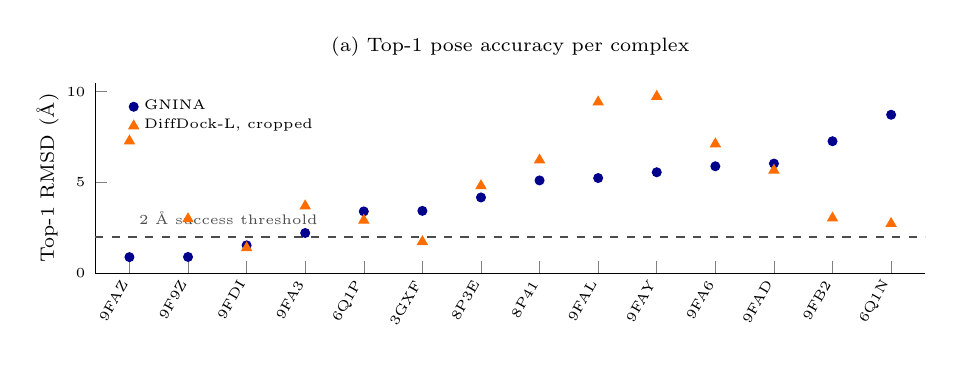
\begin{tikzpicture}
\begin{axis}[
    width=\linewidth, height=4.0cm,
    ymin=0, ymax=10.5,
    ylabel={Top-1 RMSD (\AA)},
    ylabel style={font=\scriptsize, yshift=-4pt},
    symbolic x coords={9FAZ,9F9Z,9FDI,9FA3,6Q1P,3GXF,8P3E,8P41,9FAL,9FAY,9FA6,9FAD,9FB2,6Q1N},
    xtick={9FAZ,9F9Z,9FDI,9FA3,6Q1P,3GXF,8P3E,8P41,9FAL,9FAY,9FA6,9FAD,9FB2,6Q1N},
    x tick label style={rotate=60, anchor=east, font=\tiny},
    tick label style={font=\tiny},
    axis lines*=left,
    enlarge x limits=0.045,
    title={\scriptsize (a) Top-1 pose accuracy per complex},
    legend style={font=\tiny, at={(0.03,0.97)}, anchor=north west, draw=none, fill=none, row sep=-2pt},
    legend cell align=left,
    clip=false,
]
\addplot[only marks, mark=*, mark size=1.6pt, blue!55!black] coordinates {
 (9FAZ,0.88) (9F9Z,0.89) (9FDI,1.53) (9FA3,2.21) (6Q1P,3.40) (3GXF,3.43) (8P3E,4.17) (8P41,5.11) (9FAL,5.24) (9FAY,5.56) (9FA6,5.89) (9FAD,6.04) (9FB2,7.27) (6Q1N,8.73)
};
\addlegendentry{GNINA}
\addplot[only marks, mark=triangle*, mark size=2.0pt, orange!85!red] coordinates {
 (9FAZ,7.28) (9F9Z,2.99) (9FDI,1.39) (9FA3,3.70) (6Q1P,2.91) (3GXF,1.73) (8P3E,4.81) (8P41,6.23) (9FAL,9.43) (9FAY,9.74) (9FA6,7.12) (9FAD,5.67) (9FB2,3.03) (6Q1N,2.73)
};
\addlegendentry{DiffDock-L, cropped}
\draw[dashed, thick, black!70] ({rel axis cs:0,0} |- {axis cs:9FAZ,2}) -- ({rel axis cs:1,0} |- {axis cs:9FAZ,2});
\node[anchor=south west, font=\tiny, black!70] at (axis cs:9FAZ,2.15) {2~\AA\ success threshold};
\end{axis}
\end{tikzpicture}
\end{minipage}
\hfill
\begin{minipage}{0.42\linewidth}
\centering
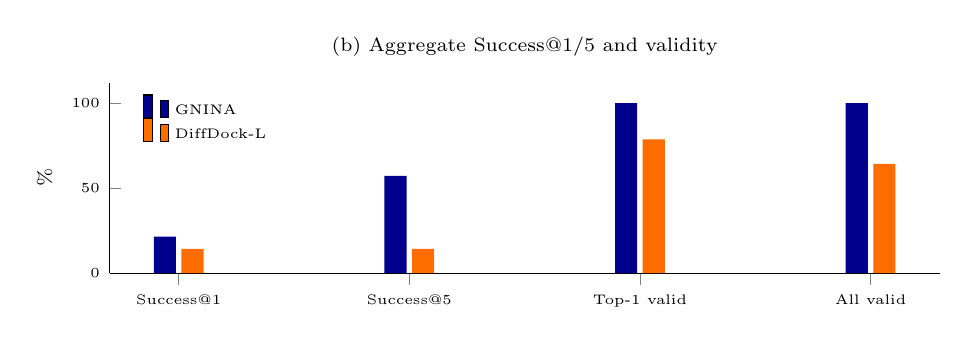
\begin{tikzpicture}
\begin{axis}[
    width=\linewidth, height=4.0cm,
    ybar, bar width=8pt,
    ymin=0, ymax=112,
    ylabel={\%},
    ylabel style={font=\scriptsize},
    symbolic x coords={Success@1,Success@5,Top-1 valid,All valid},
    xtick={Success@1,Success@5,Top-1 valid,All valid},
    x tick label style={font=\tiny},
    tick label style={font=\tiny},
    axis lines*=left,
    title={\scriptsize (b) Aggregate Success@1/5 and validity},
    legend style={font=\tiny, at={(0.03,0.97)}, anchor=north west, draw=none, fill=none, row sep=-2pt},
    legend cell align=left,
    clip=false,
]
\addplot[fill=blue!55!black, draw=none, bar shift=-5pt] coordinates {
  (Success@1,21.4) (Success@5,57.1) (Top-1 valid,100) (All valid,100)
};
\addlegendentry{GNINA}
\addplot[fill=orange!85!red, draw=none, bar shift=5pt] coordinates {
  (Success@1,14.3) (Success@5,14.3) (Top-1 valid,78.6) (All valid,64.3)
};
\addlegendentry{DiffDock-L}
\end{axis}
\end{tikzpicture}
\end{minipage}
\caption{\textbf{Docking separates sampling, ranking, and validity} (\S2.3, \S3.2, Table~\ref{tab:redocking}). (a) Top-1 RMSD per complex (sorted by GNINA's value); the primary Success@1 endpoint is null (three discordant complexes near the 2~\AA\ threshold), but GNINA's values cluster lower and less variably overall. (b) GNINA recovers a near-native pose within five outputs more often and produces more geometry-valid poses; DiffDock-L is run with a ligand-centered 15~\AA\ crop at a five-pose budget, not native/uncropped DiffDock-L (\S2.3).}
\label{fig:docking}
\end{figure}

\subsection{Chemical qualification establishes the generator reversal; structural screening is run-sensitive}

All 146 candidate/control jobs completed and returned five poses; 16 candidates (15 GenMol, 1 MolMIM) achieved the frozen Top-1 structural-proxy pass, giving a final end-to-end yield of 5.00\% (95\% exact CI 2.83--8.11\%) for GenMol versus 0.33\% (0.01--1.84\%) for MolMIM (Appendix~B); this gap is driven principally by chemical qualification, not docking, since the conditional retention estimates (15/66 vs.\ 1/3, i.e.\ 22.7\% vs.\ 33.3\%) cannot establish a generator difference with so small a MolMIM denominator. These exact binomial intervals condition on a single docking realization and do not capture ligand-embedding or run-level variability (\S3.5): a same-batch rerun did not overturn the generator ordering, but structural-proxy counts and candidate identities were run-sensitive, and the robust separation remains chemical qualification (66/300 vs.\ 3/300), not demonstrated structural discrimination. An any-pose Top-5 oracle identified 11 additional GenMol candidates (0 MolMIM), yielding 27/69 possible passes. CNN\_VS yielded 21 total passes and minimized affinity 12, versus 16 native; neither change is interpretable as better/worse qualification without candidate-level ground truth, and CNN\_VS is mechanically non-independent of the CNNaffinity-thresholded gate (\S4.1). The 16 Top-1 candidates remained primary; the 11 rescues were kept only as an exploratory reserve. The 16 primary passers occupied eight ECFP4 clusters and ten Murcko scaffolds (QED 0.53--0.78, SA 2.97--4.76, 15/16 with no Lipinski violation); predictive ADMET and exact-database-membership characterization are in Appendices~F--G.

\subsection{Paired receptor-state scores do not establish pH-dependent pharmacology}

Ambroxol's neutral-minus-acidic CNNaffinity difference was positive but small ($+0.057$), passing the one frozen, version-controlled directional sanity check. The three other docked molecules (isofagomine, P9V, P8Y) were not frozen as directional controls and instead favored the acidic receptor; only 23/57 interpretable candidate comparisons favored the neutral state. These are reported descriptively, not as a failed control check: the endpoint was never calibrated against measured pH-dependent binding, and crystallization pH, receptor-protonation, and ligand-protonation are distinct choices that two structures at different pH do not, alone, validate as a pH-dependent-binding simulation. We retain the scores as exploratory ranking information only, not evidence of pH-dependent binding, lysosomal release, or chaperoning; both receptors share an identical preparation procedure, not a controlled re-protonation (Appendix~H).

\subsection{Structural-proxy calibration is inconclusive and run-sensitive}

The preregistered cross-run comparison gave risk ratio 0.98 (95\% CI 0.81--1.21), indistinguishable from unity; after candidate rerunning exposed cross-run instability (\S3.3), the less-confounded same-batch estimate was 1.46 (0.96--2.12; Appendix~H), a weak and still-inconclusive trend rather than a confirmed effect. The rerun gave 23 GenMol and 1 MolMIM structural-proxy passers versus the frozen 15 and 1 (18/69 labels changed: 13 newly passing, 5 newly failing; 11/16 frozen passers retained). MM\_002, the sole frozen MolMIM passer, remained a passer in both runs; of the six Tranche~1 panel members (GM\_035, GM\_015, MM\_002, GM\_034, GM\_054, GM\_057), exactly 3/6 retained pass status while the other 3 (GM\_015, GM\_035, GM\_057) flipped to fail---per-candidate detail and role sensitivity in Appendix~G. CNNaffinity retained a significant size association among decoys and was the more restrictive gate component for both populations (Appendix~H, Table~\ref{tab:decoy-gate-mechanism}). Taken together, this calibrates the gate's background and run-to-run behavior, not its biological specificity; the frozen 16-candidate set and Tranche~1 panel remain unchanged, but the three flipped Tranche~1 members should be treated as requiring experimental confirmation, not dropped retrospectively.

Across the candidate-screen and redocking audits, ligand preparation run at different times produced different starting conformers despite an explicitly fixed RDKit seed, changing 18/69 candidate-screen labels and 3/14 redocking Success@1 verdicts (Figure~\ref{fig:stability}). Conformer preparation was therefore an uncontrolled experimental variable in this deployed pipeline, not the deterministic preprocessing detail it is usually treated as. Before assigning a cause, we diagnosed the actual call path: the frozen pipeline uses \texttt{AllChem.EmbedMolecule}, not \texttt{EmbedMultipleConfs}, so RDKit's \texttt{numThreads} parameter---which defaults to 1 and is never overridden here---is not in play, and \texttt{randomSeed} is the only ETKDGv3 default this code overrides. A targeted diagnostic (Appendix~D) found this exact embedding step to be exactly reproducible, both within one process and across independent fresh-process invocations, within one fixed environment. Conformer preparation is therefore established as a plausible major source of the observed instability, but this is not confirmed as RDKit's seeded embedding being inherently or universally nondeterministic, nor as the sole cause: machine and build identity were not recorded across occasions, so environment drift remains an open, unconfirmed alternative explanation.

\begin{figure}[t]
\centering
\begin{minipage}{0.55\linewidth}
\centering
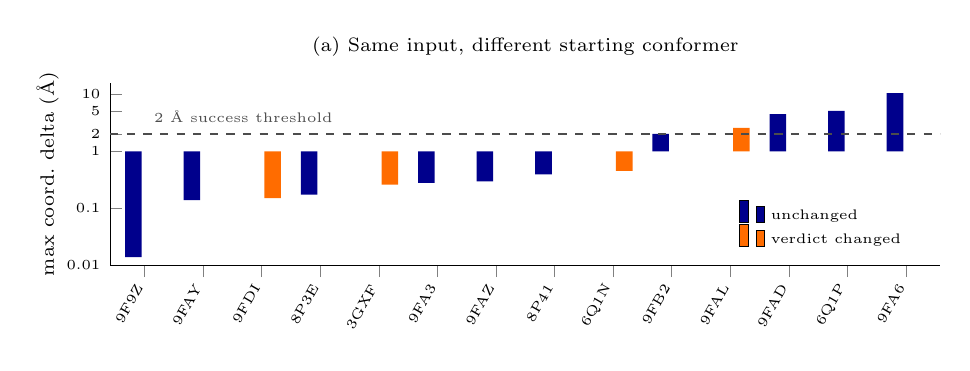
\begin{tikzpicture}
\begin{axis}[
    width=\linewidth, height=3.9cm,
    ymode=log,
    ymin=0.01, ymax=16,
    ytick={0.01,0.1,1,2,5,10},
    yticklabels={0.01,0.1,1,2,5,10},
    ylabel={max coord.\ delta (\AA)},
    ylabel style={font=\scriptsize, yshift=-4pt},
    symbolic x coords={9F9Z,9FAY,9FDI,8P3E,3GXF,9FA3,9FAZ,8P41,6Q1N,9FB2,9FAL,9FAD,6Q1P,9FA6},
    xtick={9F9Z,9FAY,9FDI,8P3E,3GXF,9FA3,9FAZ,8P41,6Q1N,9FB2,9FAL,9FAD,6Q1P,9FA6},
    x tick label style={rotate=60, anchor=east, font=\tiny},
    tick label style={font=\tiny},
    ybar, bar width=6pt,
    axis lines*=left,
    enlarge x limits=0.045,
    title={\scriptsize (a) Same input, different starting conformer},
    legend style={font=\tiny, at={(0.97,0.03)}, anchor=south east, draw=none, fill=none, row sep=-2pt},
    legend cell align=left,
    clip=false,
]
\addplot[draw=none, fill=blue!55!black] coordinates {
 (9F9Z,0.0138) (9FAY,0.139) (8P3E,0.1736) (9FA3,0.2791) (9FAZ,0.2956) (8P41,0.3913) (9FB2,2.0229) (9FAD,4.4925) (6Q1P,5.1249) (9FA6,10.493)
};
\addlegendentry{unchanged}
\addplot[draw=none, fill=orange!85!red] coordinates {
 (9FDI,0.151) (3GXF,0.2584) (6Q1N,0.4546) (9FAL,2.5649)
};
\addlegendentry{verdict changed}
\draw[dashed, thick, black!70] ({rel axis cs:0,0} |- {axis cs:9F9Z,2}) -- ({rel axis cs:1,0} |- {axis cs:9F9Z,2});
\node[anchor=south west, font=\tiny, black!70] at (axis cs:9F9Z,2.15) {2~\AA\ success threshold};
\end{axis}
\end{tikzpicture}
\end{minipage}
\hfill
\begin{minipage}{0.42\linewidth}
\centering
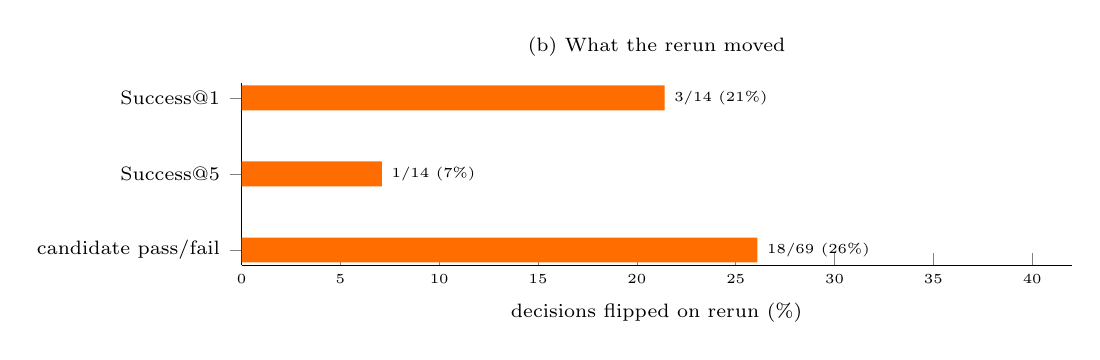
\begin{tikzpicture}
\begin{axis}[
    width=\linewidth, height=3.9cm,
    xbar, bar width=9pt,
    xmin=0, xmax=42,
    xlabel={decisions flipped on rerun (\%)},
    xlabel style={font=\scriptsize},
    symbolic y coords={candidate pass/fail,Success@5,Success@1},
    ytick=data,
    y tick label style={font=\scriptsize},
    tick label style={font=\tiny},
    axis lines*=left,
    title={\scriptsize (b) What the rerun moved},
    clip=false,
]
\addplot[fill=orange!85!red, draw=none] coordinates {
  (21.4,Success@1) (7.1,Success@5) (26.1,candidate pass/fail)
};
\node[anchor=west, font=\tiny] at (axis cs:21.4,Success@1) {3/14 (21\%)};
\node[anchor=west, font=\tiny] at (axis cs:7.1,Success@5) {1/14 (7\%)};
\node[anchor=west, font=\tiny] at (axis cs:26.1,candidate pass/fail) {18/69 (26\%)};
\end{axis}
\end{tikzpicture}
\end{minipage}
\caption{\textbf{Stability by determinism class} (\S3.2, \S3.5, Appendix~D). (a) Maximum all-atom coordinate difference between the frozen redocking-benchmark inputs and a fresh-embedding rerun of the identical pipeline (same seed, same code); 5/14 exceed the benchmark's own 2~\AA\ success threshold, and verdict changes (orange) do not track perturbation size (9FDI flips on 0.15~\AA\ while 9FA6 moves 10.49~\AA\ and does not). (b) Share of decisions that changed on the same-batch reruns above; chemical gates (0\%, not shown) are pure functions of the molecular graph and are unaffected by construction.}
\label{fig:stability}
\end{figure}

\subsection{A weaker model's violation rate falls once evidence-semantics rules are stated at all, not with each further step of formalization}

\begin{table}[t]
  \caption{Agent compliance with pre-specified calibrated answers, 6 conditions (Sonnet 5: 5 replicate runs each; Haiku 4.5: 50 replicate runs each), 10 items per run (\S2.4, Appendix~I).}
  \label{tab:agent-probe}
  \centering
  \footnotesize
  \begin{tabular}{llrl}
    \toprule
    Model & Prompt condition & Item-2 compliant & All other 9 items \\
    \midrule
    Sonnet 5 & Free-form & 5/5 & 45/45 compliant \\
    Sonnet 5 & Prose guidance & 5/5 & 45/45 compliant \\
    Sonnet 5 & Explicit contract & 5/5 & 45/45 compliant (rule-cited) \\
    Haiku 4.5 & Free-form & 18/50 & 450/450 compliant \\
    Haiku 4.5 & Prose guidance & 33/50 & 450/450 compliant \\
    Haiku 4.5 & Explicit contract & 36/50 & 450/450 compliant (rule-cited) \\
    \bottomrule
  \end{tabular}
\end{table}

An earlier, single-run version of this probe (one instance per condition, System A vs.\ System B only) found Sonnet 5 compliant in both conditions and Haiku 4.5 compliant in the contract condition but not in free-form. A single separate instance per condition cannot distinguish a real prompt effect from ordinary stochastic variation across LLM samples, and cannot tell whether simply stating the same facts as prose (no rule numbers, no citation requirement) would do just as well as the formalized contract. We therefore expanded the probe to 5 instances per condition and added System B-prose to check both (Appendix~I); when that n=5 design still could not clear significance (Fisher's exact $p=0.52$ at best), we scaled Haiku, the only condition showing variation, to 50 replicates per condition (Sonnet stayed at n=5: a clean 15/15 ceiling has no variance left to resolve).

Table~\ref{tab:agent-probe} summarizes the outcome, and it is more informative than the original pairing. Across all 1,650 graded responses, 9 of the 10 items are answered correctly in every single run, regardless of model or prompt condition (1,485/1,485); the CI-crosses-1 item (Table~\ref{tab:decoy-gate-mechanism}-style reasoning) and the prediction-vs-measurement item are followed with no exceptions even by the free-form weaker model, so a single sharp statistical rule needs no scaffolding to be respected. The one item with any variation is the redocking item built from Table~\ref{tab:redocking} (Docking Tool Superiority): the primary Top-1 comparison (3/14 vs.\ 2/14) is not significant, and the correct answer treats the larger secondary Top-5 gap (8/14 vs.\ 2/14) as suggestive, not as grounds to declare one tool practically superior. Sonnet 5 gets this right in all 15 of its runs, across all three prompt conditions---a replicated ceiling effect, not a lucky draw. Haiku 4.5 does not: its violation rate on this one item falls from 64\% under the free-form baseline, which states no rules (many runs conclude something like ``Tool X appears better for practical use\ldots despite the top-1 equivalence,'' using the secondary metric to resolve the null primary one), to 34\% once the same eight rules are stated as unformalized prose guidance, to 28\% under the formalized, rule-cited contract representation of those same rules---and only on this item: the contract is not a generic accuracy booster, its value concentrates on the one evidence-hierarchy pattern it was written to guard against.

Three things follow that the original n=5 pairing could not show. First, the violation is real and recurrent, not a small-sample artifact: 32 of 50 free-form Haiku runs make it. Second, the overall trend is now significant (free-form 18/50 vs.\ contract 36/50, Fisher's exact $p=0.0006$; trend test $p=0.00027$). Third---the finding that survived replication rather than the one we expected---the effect is not the even, three-step staircase the $n=5$ data suggested: nearly all of the improvement occurs between free-form and \emph{any} explicit statement of the rules (prose, 33/50; $p=0.0048$ vs.\ free-form), while the further step to the numbered, rule-cited contract (36/50) is not distinguishable from noise ($p=0.67$; Appendix~I). We therefore do not claim, as the $n=5$ data suggested, that formalizing guidance into a contract meaningfully helps beyond stating the same facts in prose; the larger sample supports only the more modest claim that stating the relevant considerations at all substantially reduces this failure. We still do not claim the contract \emph{causes} compliance on any run---an associational rate, not a controlled intervention. Independent of accuracy, the structural finding holds: every Sonnet 5 contract-condition response carries an explicit, per-item rule citation the equally-correct free-form and prose responses do not---an auditable trail a reviewer would need to check an agent's reasoning, not only its answer---though the trail is not self-correcting: on Haiku 4.5's own 14 contract-condition failures, a rule number is always cited but never R5 (Appendix~I). This probes whether an agent can operationalize a supplied evidence-semantics contract, not whether such contracts improve general scientific reasoning on unrelated tasks (Appendix~I).

\section{Discussion}

\subsection{The relevant comparison depends on the decision}

Together, the experiments separate robust conclusions from provisional signals. MolMIM better supported broad exploration (uniqueness, diversity, QED, SA), while GenMol's analogue-focused configuration better satisfied the frozen contract---configuration--contract fit, not generator superiority (Figure~\ref{fig:funnel}). In redocking, Top-1 performance was unresolved between the two tools, but under the five-pose budget GNINA achieved better pose recovery and geometry validity than cropped DiffDock-L (Figure~\ref{fig:docking})---a supporting audit feeding the candidate screen, not an independent claim about which docking tool is generally better (\S4.2). The 15/300-versus-1/300 downstream screening yield reflects chemical qualification, not demonstrated structural discrimination between the generators. The frozen 16 compounds are therefore best understood as an auditable prioritization set, not as validated GCase binders, pharmacological chaperones, or confirmed hits.

The practical lesson is therefore three-part: freeze the decision contract for honest tool comparison; treat every advancement proxy---and, per Figure~\ref{fig:stability}, the ligand-preparation step that feeds it---as an experimental factor needing calibration before it is trusted to advance compounds; and, per Table~\ref{tab:agent-probe}, write the contract down explicitly: on the one task where a weaker agent's violation rate was substantial free-form (64\%, 50 runs), stating the facts explicitly---prose or contract---roughly halved it (34\%/28\%, both significant vs.\ free-form; \S3.6), though prose-to-contract itself was not significant---while a stronger, already-correct agent still gained an auditable reason for each conclusion in all 15 runs. For GCase, the next cycle should assay the frozen Tranche~1 panel for binding, stabilization, and pH-resolved catalytic modulation; use those outcomes to select accurate, reproducible docking--scoring--ranking combinations; and only then validate a new candidate batch prospectively.

\subsection{Limitations}

One contract, one target, two generators, two dockers support no general claim about these tools; the methodology is general, the case study an existence proof. The docking comparison carries a disclosed asymmetry favoring GNINA (\S2.2: a crystal-ligand-shaped box vs.\ DiffDock-L's isotropic 15~\AA\ crop), so Table~\ref{tab:redocking} is not a claim about native DiffDock-L. The redocking set is allosteric-heavy (11/14) while the candidate-screen gate is active-site-only, so GNINA's more frequent near-native recovery here does not by itself make it the better selector for generated candidates; the active-site subset (\emph{n}=3, Appendix~D) is too small to resolve this independently. The embedding rerun is a single additional realization, not a variance estimate; machine/build identity was not recorded, so its non-reproducibility's cause remains open (Appendix~D). A purchasable-catalogue retrieval comparator now runs at the chemical level (\S3.1, Appendix~J: 258/300 vs.\ 66/300), but not structurally, since this project's own run-sensitivity (\S3.5) makes comparing it against the frozen 15/300 and 1/300 yields unsafe without a same-batch rerun; separately, only 1/16 candidates returned an exact-match ZINC in-stock hit (Appendix~G), a narrower question. The experimental panel is pre-data. The agent probe (\S2.4, \S3.6, Appendix~I) is a one-shot batch of ten interpretation questions answered by a memory-free general-purpose agent, not an autonomous, multi-step, tool-using agent loop; the rubric was checked against a blinded second rater covering the full n=165 sample (157/165 agreement, $\kappa$ 0.89--0.92 across the two batches; Appendix~I), and the significance results below are unchanged under the blind-graded counts. The failure mode recurs and falls significantly from free-form to either guided condition ($p=0.0006$; trend $p=0.00027$), but prose-to-contract is not significant ($p=0.67$), and none of this shows the contract \emph{causes} compliance on a given run. Only two models were tested; adopting a contract needs labels we lack (MolDockLab~[14]).

\section*{References}

\small

[1] Polykovskiy, D. et al. Molecular Sets (MOSES): A Benchmarking Platform for Molecular Generation Models. \textit{Frontiers in Pharmacology} 11, 565644 (2020). \url{https://doi.org/10.3389/fphar.2020.565644}

[2] Brown, N., Fiscato, M., Segler, M. H. S. \& Vaucher, A. C. GuacaMol: Benchmarking Models for De Novo Molecular Design. \textit{Journal of Chemical Information and Modeling} 59, 1096--1108 (2019). \url{https://doi.org/10.1021/acs.jcim.8b00839}

[3] Buttenschoen, M., Morris, G. M. \& Deane, C. M. PoseBusters: AI-based docking methods fail to generate physically valid poses or generalise to novel sequences. \textit{Chemical Science} 15, 3130--3139 (2024). \url{https://doi.org/10.1039/D3SC04185A}

[4] McNutt, A. T. et al. GNINA 1.0: molecular docking with deep learning. \textit{Journal of Cheminformatics} 13, 43 (2021). \url{https://doi.org/10.1186/s13321-021-00522-2}

[5] Corso, G., St\"ark, H., Jing, B., Barzilay, R. \& Jaakkola, T. DiffDock: Diffusion Steps, Twists, and Turns for Molecular Docking. \textit{International Conference on Learning Representations} (2023). \url{https://openreview.net/forum?id=kKF8_K-mBbS}

[6] Corso, G. et al. Deep Confident Steps to New Pockets: Strategies for Docking Generalization. \textit{International Conference on Learning Representations} (2024). \url{https://openreview.net/forum?id=UfBIxpTK10}

[7] Maegawa, G. H. B. et al. Identification and Characterization of Ambroxol as an Enzyme Enhancement Agent for Gaucher Disease. \textit{Journal of Biological Chemistry} 284, 23502--23516 (2009). \url{https://doi.org/10.1074/jbc.M109.012393}

[8] Bendikov-Bar, I., Maor, G., Filocamo, M. \& Horowitz, M. Ambroxol as a pharmacological chaperone for mutant glucocerebrosidase. \textit{Blood Cells, Molecules, and Diseases} 50, 141--145 (2013). \url{https://doi.org/10.1016/j.bcmd.2012.10.007}

[9] Lee, S. et al. GenMol: A Drug Discovery Generalist with Discrete Diffusion. arXiv:2501.06158 (2025). \url{https://arxiv.org/abs/2501.06158}

[10] Reidenbach, D., Livne, M., Ilango, R. K., Gill, M. \& Israeli, J. Improving Small Molecule Generation using Mutual Information Machine. arXiv:2208.09016 (2022). \url{https://arxiv.org/abs/2208.09016}

[11] Wei, R. R. et al. X-ray and Biochemical Analysis of N370S Mutant Human Acid $\beta$-Glucosidase. \textit{Journal of Biological Chemistry} 286, 299--308 (2011). \url{https://doi.org/10.1074/jbc.M110.150060}

[12] Swanson, K. et al. ADMET-AI: a machine learning ADMET platform for evaluation of large-scale chemical libraries. \textit{Bioinformatics} 40, btae416 (2024). \url{https://doi.org/10.1093/bioinformatics/btae416}

[13] Medina, J. \& White, A. D. Bloom filters for molecules. \textit{Journal of Cheminformatics} 15, 95 (2023). \url{https://doi.org/10.1186/s13321-023-00765-1}

[14] Agha, H. et al. Data driven selection of consensus docking pipelines for structure based hit identification. \textit{npj Drug Discovery} 3, 37 (2026). \url{https://doi.org/10.1038/s44386-026-00063-4}

[15] Su, M., Yang, Q., Du, Y., Feng, G., Liu, Z., Li, Y. \& Wang, R. Comparative Assessment of Scoring Functions: The CASF-2016 Update. \textit{Journal of Chemical Information and Modeling} 59, 895--913 (2019). \url{https://doi.org/10.1021/acs.jcim.8b00545}

[16] Gao, W. \& Coley, C. W. The Synthesizability of Molecules Proposed by Generative Models. \textit{Journal of Chemical Information and Modeling} 60, 5714--5723 (2020). \url{https://doi.org/10.1021/acs.jcim.0c00174}

[17] Tripp, A., Simm, G. N. C. \& Hern\'{a}ndez-Lobato, J. M. A Fresh Look at De Novo Molecular Design Benchmarks. \textit{NeurIPS 2021 AI for Science Workshop} (2021). \url{https://openreview.net/forum?id=gS3XMun4cl_}

[18] W\'{o}jcikowski, M., Ballester, P. J. \& Siedlecki, P. Performance of machine-learning scoring functions in structure-based virtual screening. \textit{Scientific Reports} 7, 46710 (2017). \url{https://doi.org/10.1038/srep46710}

[19] Boiko, D. A., MacKnight, R., Kline, B. \& Gomes, G. Autonomous chemical research with large language models. \textit{Nature} 624, 570--578 (2023). \url{https://doi.org/10.1038/s41586-023-06792-0}

[20] M. Bran, A., Cox, S., Schilter, O., Baldassari, C., White, A. D. \& Schwaller, P. Augmenting large language models with chemistry tools. \textit{Nature Machine Intelligence} 6, 525--535 (2024). \url{https://doi.org/10.1038/s42256-024-00832-8}

\clearpage
\appendix

These appendices are supplementary material and are not counted against the nine-page main-text limit. All raw manifests, per-run logs, candidate structures, hashes, and code referenced below are version-controlled in the project repository; the tables here are condensed, verified extracts. Repository: \url{https://github.com/lifeai-io/DecisionBench-DD}.

\FloatBarrier
\section{Generator configurations and replicate-level metrics}
\label{app:a}

\textbf{Frozen invocation parameters.} Both tools received the identical seed SMILES \texttt{C1=C(C(=C(C=C1Br)Br)N)CNC2CCC(CC2)O} and were called three times as independent replicates (100 molecules requested per call); neither API exposes a documented random-seed field.

\begin{table}[h]
\centering
\footnotesize
\begin{tabular}{ll}
\toprule
GenMol NIM parameter & Value \\
\midrule
num\_molecules & 100 (per replicate) \\
temperature & 1.0 (documented default) \\
noise & 1.0 (documented default) \\
gamma & 0.0 \\
min\_add\_len & 24 \\
scoring & QED \\
unique / filter & false / false (post-hoc filtering done by our own gates, not the API) \\
\bottomrule
\end{tabular}
\hspace{1em}
\begin{tabular}{ll}
\toprule
MolMIM NIM parameter & Value \\
\midrule
num\_molecules & 100 (per replicate) \\
algorithm & CMA-ES \\
property\_name & QED \\
minimize & false \\
min\_similarity & 0.3 (requested; \S2.1 notes this was not observed as a hard floor) \\
particles & 100 \\
iterations & 10 \\
\bottomrule
\end{tabular}
\end{table}

\textbf{Per-replicate breakdown} (100 requested per replicate; source: \texttt{chemical\_gate\_audit.csv}):

\begin{table}[h]
\centering
\footnotesize
\begin{tabular}{lrrr}
\toprule
GenMol & Replicate 1 & Replicate 2 & Replicate 3 \\
\midrule
Valid & 100 & 100 & 100 \\
Within-replicate unique & 84 & 49 & 68 \\
Chemically qualified & 30 & 29 & 7 \\
\bottomrule
\end{tabular}
\hspace{1em}
\begin{tabular}{lrrr}
\toprule
MolMIM & Replicate 1 & Replicate 2 & Replicate 3 \\
\midrule
Valid & 97 & 100 & 100 \\
Within-replicate unique & 97 & 100 & 100 \\
Chemically qualified & 1 & 1 & 1 \\
\bottomrule
\end{tabular}
\end{table}

GenMol's 100.0\% validity has run-to-run stdev 0.0\,pp; MolMIM's 99.0\% pooled validity has stdev 1.7\,pp (driven entirely by replicate 1). Qualified counts sum to 66 (GenMol) and 3 (MolMIM), matching Table~1. GenMol replicate 3's markedly lower qualified count (7 vs.\ 30 and 29) is not explained by lower validity or uniqueness (its within-replicate uniqueness, 68, is higher than replicate 2's 49): all three replicate request manifests returned HTTP 200 with the full 100 records requested and no logged error or anomaly, so this is reported as unexplained run-to-run variance from the hosted service, not a diagnosed cause. Because this drives the between-replicate spread underlying the cluster-bootstrap CI above, we flag it explicitly rather than let a single unexplained low replicate pass without comment.

\textbf{Summed vs.\ pooled uniqueness.} GenMol's within-replicate unique counts sum to $84+49+68=201$, matching the ``67.0\% unique'' figure reported in Table~1. This is \emph{not} the same as the number of distinct molecules across all three replicates pooled together: recomputing uniqueness over the union of all three GenMol replicates gives \textbf{200} distinct canonical structures, i.e.\ exactly one molecule recurred across two different replicates. To be precise about what each number drives: $Y_{\mathrm{chemical}} = N_{\mathrm{pass\ all\ gates}}/N_{\mathrm{requested}}$ always has a fixed denominator of 300 requested molecules; within-replicate deduplication is one of the cumulative gates that determines which outputs can reach the numerator, not a component of the denominator. The pooled count (200) is reported here only as a diagnostic and was not used in any gate or headline statistic.

\textbf{MolMIM \texttt{min\_similarity} sensitivity (post-hoc, reviewer-requested).} Run after inspecting the primary results, using the identical seed, pipeline, and frozen gates but overriding only \texttt{min\_similarity} (\texttt{decisionbench\_dd\_eval/run\_generation\_sensitivity.py}; source manifests in \texttt{runs\_sensitivity/}, scored results in \texttt{results\_sensitivity/}):

\begin{table}[h]
\centering
\footnotesize
\begin{tabular}{lrrrrr}
\toprule
\texttt{min\_similarity} & Rep.\ 1 & Rep.\ 2 & Rep.\ 3 & Pooled qualified & Yield (95\% CI) \\
\midrule
0.3 (primary) & 1 & 1 & 1 & 3/300 & 1.0\% (0.0--2.3\%) \\
0.5 & 1 & 1 & 0 & 2/300 & 0.7\% (0.0--1.7\%) \\
0.7 & 4 & 1 & 5 & 10/300 & 3.3\% (1.3--5.3\%) \\
\bottomrule
\end{tabular}
\caption{MolMIM chemically-qualified counts (of 100 requested per replicate) as \texttt{min\_similarity} varies. Median externally-recomputed ECFP4 Tanimoto-to-seed was 0.167 at all three settings, consistent with the primary-run finding that this parameter does not impose a hard similarity floor under our independent RDKit recomputation. GenMol's pooled qualified yield (22.0\%, unaffected by this rerun) remains far above MolMIM's at every tested setting.}
\end{table}

\textbf{Sensitivity scorecard (distributional detail).} Table~4 reports only pass/fail counts; the observed generated-molecule distributions differed across the requested settings, most visibly in the upper tail:

\begin{table}[h]
\centering
\footnotesize
\begin{tabular}{lrr}
\toprule
Metric & \texttt{0.5} & \texttt{0.7} \\
\midrule
Valid & 295/300 & 297/300 \\
Unique among valid & 100.0\% & 99.7\% \\
Mean ECFP4 similarity & 0.170 & 0.178 \\
Median ECFP4 similarity & 0.167 & 0.167 \\
Frozen similarity-band pass & 4/300 & 14/300 \\
Maximum similarity & 0.458 & 0.468 \\
Mean QED & 0.755 & 0.783 \\
Mean SA & 3.34 & 3.17 \\
Internal diversity & 0.839 & 0.837 \\
Chemical pass & 2/300 & 10/300 \\
Structural-proxy pass & 0/300 & 2/300 \\
\bottomrule
\end{tabular}
\caption{Sensitivity-run distributional detail. Source: molecule-level sensitivity outputs in the project repository. Median externally recomputed ECFP4 similarity was 0.167 at both settings. The observed \texttt{0.7} sample had higher mean and maximum similarity than the \texttt{0.5} sample, but without controlled seeds this descriptive difference cannot be attributed to \texttt{min\_similarity}. No output reached external ECFP4 similarity 0.5 or 0.7 (maximum observed 0.468).}
\end{table}

\FloatBarrier

\textbf{End-to-end GNINA re-screen of the sensitivity candidates.} The 2 (\texttt{min\_similarity=0.5}) and 10 (\texttt{0.7}) qualified candidates above were carried through the identical candidate-screen pipeline (\S2.3: same digest-pinned GNINA image, boxes, gate; \texttt{decisionbench\_dd\_docking/prepare\_candidate\_screen\_ligands.py} / \texttt{run\_candidate\_screen\_gnina.py} / \texttt{score\_candidate\_screen.py}, run on a separate GPU machine from the primary screen):

\begin{table}[h]
\centering
\footnotesize
\begin{tabular}{lrr}
\toprule
\texttt{min\_similarity} & Structural-proxy pass & End-to-end yield (95\% CI) \\
\midrule
0.3 (primary) & 1/300 & 0.33\% (0.01--1.84\%) \\
0.5 & 0/300 & 0.00\% (0.00--1.22\%) \\
0.7 & 2/300 & 0.67\% (0.08--2.39\%) \\
\midrule
GenMol (fixed, unaffected) & 15/300 & 5.00\% (2.83--8.11\%) \\
\bottomrule
\end{tabular}
\caption{End-to-end structural-proxy yield of the MolMIM sensitivity candidates. Source: candidate-screen sensitivity outputs in the project repository, against GenMol's frozen primary yield (unaffected by this rerun, since only MolMIM was regenerated). The two \texttt{0.7} structural passers are post-hoc sensitivity outputs only and were not added to the frozen 16-candidate primary set characterized in \S3.3 and Appendices E--G. GenMol's frozen 15/300 yield remained higher than MolMIM's 0/300 and 2/300 sensitivity yields at every tested \texttt{min\_similarity} setting. The re-scored Ambroxol threshold differed from the primary value by 0.0009, a small cross-run difference whose source was not isolated in that comparison. This difference was smaller than every candidate's pass/fail margin and changed no classification; a larger-scale post-hoc test (Appendix~H) found a substantially bigger effect for the full 69-candidate population, with ligand-embedding identified as a plausible major contributor alongside (not necessarily instead of) GPU-hardware variance, so this narrow result should not be generalized.}
\end{table}

\FloatBarrier
\section{Chemical-gate definitions and attrition audit}
\label{app:b}

\textbf{Gate order and thresholds} (frozen protocol v1.2, \texttt{qualification\_gates\_v1.0.json}): valid (RDKit parses) $\to$ unique (first occurrence within its own replicate) $\to$ not an exact Ambroxol copy $\to$ ECFP4 Tanimoto to seed in $[0.30,0.95)$ (radius 2, 2048-bit) $\to$ QED $\geq 0.50$ $\to$ SA (Ertl) $\leq 5.0$ $\to$ MW $200$--$550$~Da $\to$ cLogP $0$--$5$ $\to$ TPSA $\leq 100$~\AA$^2$ $\to$ zero PAINS\_A/B/C hits (absolute gate) $\to$ no new, unmapped Brenk alert instance.

\textbf{Seed-relative Brenk rule.} Ambroxol itself triggers an aniline Brenk alert, so a candidate's Brenk occurrence is disqualifying only if it does \emph{not} correspond, atom-for-atom, to the seed's own alert instance. Correspondence is computed via \texttt{rdFMCS.FindMCS} (atom compare: elements; bond compare: order; ring-matches-ring-only) between seed and candidate, and a candidate occurrence is seed-inherited only if every atom of some seed instance maps under this correspondence to exactly the candidate's matched atom set. This instance-level rule (v1.2) replaced an earlier, alert-\emph{type}-only rule (v1.1) that could not distinguish the seed's own aniline from an unrelated second aniline introduced elsewhere; both amendments were made from the seed molecule alone, before any GenMol/MolMIM comparison data existed.

\begin{table}[h]
\centering
\footnotesize
\begin{tabular}{lrrrr}
\toprule
Stage (cumulative) & \multicolumn{2}{c}{GenMol} & \multicolumn{2}{c}{MolMIM} \\
 & count & \% of 300 & count & \% of 300 \\
\midrule
Requested & 300 & 100.0\% & 300 & 100.0\% \\
Valid & 300 & 100.0\% & 297 & 99.0\% \\
Unique (within replicate) & 201 & 67.0\% & 297 & 99.0\% \\
Not exact seed & 199 & 66.3\% & 297 & 99.0\% \\
Similarity band [0.30, 0.95) & 148 & 49.3\% & 12 & 4.0\% \\
QED $\geq$0.50 & 87 & 29.0\% & 11 & 3.7\% \\
SA $\leq$5.0 & 84 & 28.0\% & 11 & 3.7\% \\
MW 200--550~Da & 83 & 27.7\% & 11 & 3.7\% \\
cLogP 0--5 & 70 & 23.3\% & 9 & 3.0\% \\
TPSA $\leq$100~\AA$^2$ & 68 & 22.7\% & 8 & 2.7\% \\
No PAINS & 68 & 22.7\% & 8 & 2.7\% \\
\textbf{Chemically qualified} & \textbf{66} & \textbf{22.0\%} & \textbf{3} & \textbf{1.0\%} \\
\bottomrule
\end{tabular}
\caption{Full attrition funnel underlying Table~1 (pooled across the three replicates per tool). Source: \texttt{chemical\_gate\_audit.csv} / \texttt{results/summary.md}.}
\label{tab:attrition-funnel}
\end{table}

Brenk instance rates (of valid molecules): GenMol -- any alert 100.0\%, all-seed-inherited 84.3\%, $\geq$1 new/unmapped instance (used for qualification) 15.7\%. MolMIM -- any alert 51.2\%, all-seed-inherited 0.3\%, $\geq$1 new instance 50.8\%.

\textbf{Marginal (independent) per-gate pass rates.} The cumulative funnel above conflates gate stringency with gate position: a gate applied late only screens molecules that already survived every earlier gate. Each gate is in fact evaluated independently per molecule (\texttt{decisionbench\_dd\_eval/gates.py:evaluate\_gates}, not short-circuited), so the marginal pass rate of every gate against the full valid population is recoverable directly from \texttt{results/molecule\_level.csv} without rerunning anything:

\begin{table}[h]
\centering
\footnotesize
\begin{tabular}{lrr}
\toprule
Gate (applied independently) & GenMol (\% of 300 valid) & MolMIM (\% of 297 valid) \\
\midrule
Within-replicate unique & 67.0\% & 100.0\% \\
Not exact seed & 99.3\% & 100.0\% \\
Similarity $\geq$0.30 & \textbf{76.7\%} & \textbf{4.0\%} \\
Similarity $<$0.95 & 99.3\% & 100.0\% \\
QED $\geq$0.50 & \textbf{61.7\%} & \textbf{97.0\%} \\
SA $\leq$5.0 & 97.7\% & 100.0\% \\
MW 200--550~Da & 98.7\% & 100.0\% \\
cLogP 0--5 & 69.0\% & 97.0\% \\
TPSA $\leq$100~\AA$^2$ & 97.7\% & 97.3\% \\
No PAINS & 99.7\% & 99.3\% \\
No new Brenk instance & 84.3\% & 49.2\% \\
\midrule
\textbf{Cumulative final qualified} & \textbf{22.0\%} & \textbf{1.0\%} \\
\bottomrule
\end{tabular}
\caption{Marginal per-gate pass rate (each gate scored alone against all valid outputs, not against survivors of earlier gates), versus the cumulative funnel in Table~\ref{tab:attrition-funnel}. The similarity gate alone rejects 96\% of MolMIM's valid outputs (4.0\% marginal pass) while rejecting only 23\% of GenMol's (76.7\%); QED alone shows the opposite pattern (97.0\% vs.\ 61.7\%). The largest marginal separation occurs at the similarity gate, although the seed-relative Brenk gate also contributes (84.3\% vs.\ 49.2\%).}
\label{tab:pergate}
\end{table}

\textbf{End-to-end candidate yield.} Continuing the funnel above through docking (\S2.3) to the frozen structural-pass gate (\S3.3):

\begin{table}[h]
\centering
\footnotesize
\begin{tabular}{lrr}
\toprule
Stage & GenMol & MolMIM \\
\midrule
Requested & 300 & 300 \\
Chemically qualified & 66 (22.0\%) & 3 (1.0\%) \\
Primary structural-proxy pass & 15 & 1 \\
Conditional structural retention & 22.7\% & 33.3\% \\
\textbf{Final yield, 95\% exact CI} & \textbf{5.00\% (2.83--8.11\%)} & \textbf{0.33\% (0.01--1.84\%)} \\
\bottomrule
\end{tabular}
\caption{End-to-end candidate yield (conditional retention shown separately; MolMIM denominator is only three). Summarized in the main text, \S3.3. Exact binomial intervals quantify molecule-level variation conditional on the frozen docking realization; they do not include embedding or run-level variability (\S3.5, Appendix~H).}
\end{table}

\FloatBarrier
\section{14-complex structural-validation set and preparation provenance}
\label{app:c}

\begin{table}[h]
\centering
\footnotesize
\begin{tabular}{lccccc}
\toprule
PDB ID & Site & Res.\ (\AA) & Ligand & RSCC & Occ.\ \\
\midrule
9F9Z & allosteric & 2.28 & A1IBI & 0.893 & 0.80 \\
9FA3 & allosteric & 1.36 & A1IBC & 0.896 & 0.62 \\
9FA6 & allosteric & 1.49 & A1IBG & 0.935 & 0.76 \\
9FAD & allosteric & 1.80 & A1IBD & 0.942 & 0.72 \\
9FAL & allosteric & 1.39 & A1IBQ & 0.972 & 0.84 \\
9FAY & allosteric & 1.40 & A1IBR & 0.967 & 0.93 \\
9FAZ & allosteric & 1.63 & A1IBP & 0.893 & 0.71 \\
9FB2 & allosteric & 1.14 & A1IBO & 0.969 & 0.93 \\
9FDI & allosteric & 1.41 & A1IB1 & 0.931 & 0.85 \\
8P3E & allosteric & 1.75 & WSI & 0.918 & 1.00 \\
8P41 & allosteric & 1.83 & WYC & 0.894 & 1.00 \\
3GXF & active-site-chaperone & 2.40 & IFM & 0.994 & 1.00 \\
6Q1N & active-site-chaperone & 2.53 & P9V & 0.842 & 1.00 \\
6Q1P & active-site-chaperone & 2.80 & P8Y & 0.922 & 1.00 \\
\bottomrule
\end{tabular}
\caption{Frozen 14-complex redocking set (RSCC/occupancy from RCSB electron-density/occupancy metadata, used for ligand-instance selection). Ligand instance chosen per case from the deposited alternate/occupancy records, not by RMSD or docking outcome.}
\end{table}

\textbf{Receptor preparation.} PDB2PQR 3.7.1, AMBER force field, PROPKA titration, pH 7.4 (single frozen physiological pH applied uniformly, not per-structure). \textbf{Ligand preparation.} dimorphite-dl 2.0.2, pH 7.4, with a frozen, content-based (not positional) microstate tie-break rule. \textbf{Docking box.} GNINA: crystal-ligand heavy-atom extent $+6$~\AA\ per side, supplied via \texttt{-{}-center\_x/y/z -{}-size\_x/y/z}. DiffDock-L: no native pocket-restriction flag exists, so its receptor input was cropped to a 15~\AA\ radius around the same box center (69--122 of 497--1988 residues retained depending on structure) -- an approximation of pocket-conditioning, explicitly not equivalent to GNINA's box search, and not native/uncropped DiffDock-L.

\FloatBarrier
\section{Pose-level redocking results and representation-artifact audit}
\label{app:d}

\textbf{Commands.} GNINA (dockerized \texttt{gnina/gnina:latest}, GPU): \texttt{gnina -r <receptor> -l <ligand> -{}-center\_x/y/z -{}-size\_x/y/z -{}-num\_modes 5 -{}-exhaustiveness 8 -{}-seed 42 -{}-cnn\_scoring rescore}. The \texttt{:latest} tag is not itself immutable, but the run manifest recorded the resolved content digest actually pulled at execution time: \texttt{gnina/gnina@sha256:9da3dc61eef272cecb60798933a9a977d028c47024845fdf1f05a941ce5e25a2} (the same digest was independently resolved for the later candidate-screen run, \S2.3). DiffDock-L (dockerized \texttt{rbgcsail/diffdock}, commit \texttt{85c49b6} of the gcorso/DiffDock repository, batch/CSV inference mode, documented defaults \texttt{inference\_steps=20}, \texttt{samples\_per\_complex=5}): \texttt{micromamba run -n diffdock python -m inference -{}-config default\_inference\_args.yaml -{}-protein\_ligand\_csv <csv> -{}-out\_dir <dir> -{}-samples\_per\_complex 5}, run inside \texttt{docker run -{}-rm -{}-gpus all rbgcsail/diffdock}. The hosted DiffDock NIM API was explicitly \emph{not} used, since its underlying checkpoint version is not independently confirmed to be DiffDock-L.

\begin{table}[h]
\centering
\footnotesize
\begin{tabular}{lc rrcc rrcc}
\toprule
 & & \multicolumn{4}{c}{GNINA} & \multicolumn{4}{c}{DiffDock-L, cropped} \\
PDB & Site & Top-1 & Best-5 & S@1 & S@5 & Top-1 & Best-5 & S@1 & S@5 \\
\midrule
9F9Z & allo & 0.89 & 0.89 & Y & Y & 2.99 & 2.66 & N & N \\
9FA3 & allo & 2.21 & 2.21 & N & N & 3.70 & 3.70 & N & N \\
9FA6 & allo & 5.89 & 1.26 & N & Y & 7.12 & 6.36 & N & N \\
9FAD & allo & 6.04 & 1.03 & N & Y & 5.67 & 4.32 & N & N \\
9FAL & allo & 5.24 & 4.76 & N & N & 9.43 & 5.97 & N & N \\
9FAY & allo & 5.56 & 5.56 & N & N & 9.74 & 5.59 & N & N(5) \\
9FAZ & allo & 0.88 & 0.87 & Y & Y & 7.28 & 6.13 & N & N(5) \\
9FB2 & allo & 7.27 & 0.82 & N & Y & 3.03 & 2.82 & N & N(5) \\
9FDI & allo & 1.53 & 1.18 & Y & Y & 1.39 & 1.39 & Y & Y \\
8P3E & allo & 4.17 & 4.17 & N & N & 4.81 & 4.72 & N & N \\
8P41 & allo & 5.11 & 5.11 & N & N & 6.23 & 5.62 & N & N \\
3GXF & active & 3.43 & 1.62 & N & Y & 1.73 & 1.73 & Y & Y \\
6Q1N & active & 8.73 & 1.49 & N & Y & 2.73 & 2.51 & N & N \\
6Q1P & active & 3.40 & 2.62 & N & N & 2.91 & 2.91 & N & N \\
\bottomrule
\end{tabular}
\caption{Per-complex RMSD (\AA) and success at RMSD $\leq$2~\AA. Parenthesized counts under DiffDock-L S@5 indicate poses affected by the sulfonamide-charge artifact (see below); ``allo''/``active'' abbreviate allosteric/active-site-chaperone.}
\end{table}

Site-stratified aggregates: GNINA allosteric ($n$=11) Success@1/5 = 27.3\%/54.5\%; GNINA active-site ($n$=3) = 0.0\%/66.7\%. DiffDock-L allosteric = 9.1\%/9.1\%; DiffDock-L active-site = 33.3\%/33.3\%. The validation set is allosteric-heavy (11/14) while the candidate screen's advancement gate is active-site-only (\S4.1), a mismatch noted as a limitation in the main text.

\textbf{Representation-artifact audit.} Three complexes (9FAY, 9FAZ, 9FB2), five poses each (15 total), had a DiffDock-L output-representation artifact: a neutral tertiary sulfonamide nitrogen assigned a spurious $+1$ formal charge. Neutralizing this charge (\texttt{rmsd.\_fix\_known\_pose\_charge\_artifact}) was necessary to restore atom correspondence for RMSD scoring; a direct programmatic comparison confirmed zero change to atomic coordinates, connectivity, stereochemical tags, or pose ranking before vs.\ after the fix. This was a targeted representation correction, not an independent stochastic replicate: under the pinned container and invocation, repeated executions produced byte-identical poses for all 14 cases, and the interface exposed no seed control, so stochastic uncertainty could not be estimated. Geometry-validity failures are independent of this artifact and reflect the frozen geometry-validity proxy (valid valence; bonded distances within 0.7--2.2~\AA; no nonbonded heavy-atom pair below 1.5~\AA): DiffDock-L's Top-1 pose is invalid for exactly 3/14 complexes (9FAL, 9FAY, 9FB2; 11/14 = 78.6\% valid, matching Table~2), while 11/14 complexes have at least one invalid pose somewhere in their five-pose set (only 9F9Z, 9FAD, and 6Q1N have all five poses geometry-valid).

\textbf{Embedding-reproducibility audit (post-hoc, prompted by the decoy-panel finding, \S3.5).} The decoy panel found that re-preparing the same candidate produced a different starting conformer despite a fixed \texttt{randomSeed=42} (candidate GM\_009, up to 1.70~\AA\ difference across two invocations). We tested whether this transfers to the primary 14-complex benchmark by re-running the frozen protonation-selection and embedding pipeline (\texttt{prepare\_ligands.py}'s unchanged logic, invoked via the new, read-only \texttt{redocking\_reembed\_rerun.py}) in a fresh process, writing to an isolated directory without touching any frozen file. The chosen protonated SMILES was unchanged for all 14 cases, but the embedded starting conformer differed from the frozen input in all 14/14 cases (max all-atom coordinate delta by case, \AA: 9F9Z 0.01, 9FAY 0.14, 9FDI 0.15, 8P3E 0.17, 3GXF 0.26, 9FAZ 0.30, 9FA3 0.28, 8P41 0.39, 6Q1N 0.45, 9FB2 2.02, 9FAL 2.56, 9FAD 4.49, 6Q1P 5.12, 9FA6 10.49); 5/14 exceed the benchmark's own 2~\AA\ success threshold. \textbf{Before assigning a cause, we diagnosed the actual call path} (\texttt{diagnose\_embedding\_determinism.py}): preparation uses \texttt{AllChem.EmbedMolecule}, not \texttt{EmbedMultipleConfs}, so RDKit's \texttt{numThreads} parameter (default 1, never overridden) does not apply here; \texttt{randomSeed} is the only ETKDGv3 default this pipeline overrides, and \texttt{useRandomCoords}/\texttt{enforceChirality}/pruning are left at their documented defaults. For three cases spanning the delta range above (9F9Z, 6Q1P, 9FA6), re-embedding with this unchanged code path was exactly reproducible both within one process and across independent fresh-process invocations (0.0~\AA\ in every trial), yet still differed from the corresponding committed frozen file by the magnitudes reported above. Embedding is therefore reproducible within one fixed environment; the discrepancy arose between the original preparation and this session's re-preparation, run at different times without recording machine identity or RDKit build details beyond the pinned package version (\texttt{rdkit==2026.3.5} in both). This does not establish RDKit's seeded embedding as inherently or universally nondeterministic, nor confirm environment drift as the cause -- only that the deployed pipeline's output was not reproduced when re-run outside its original invocation, for a reason this audit cannot fully isolate. DiffDock-L is structurally immune to this specific risk: it consumes only \texttt{docking\_input\_protonated\_smiles} (\S\ref{app:d}'s Commands paragraph), never the embedded conformer, consistent with its already-established byte-identical-rerun reproducibility above. GNINA's \texttt{-l} input does depend on the embedded conformer, so we redocked the fresh embeddings (identical frozen receptor, box, and GNINA settings, same pinned image digest as the primary run) and rescored with the existing, unmodified \texttt{evaluate\_docking.py}. Table~\ref{tab:redocking}'s GNINA numbers are \textbf{not robust} to this: Success@1 rose from 3/14 (21.4\%) to 4/14 (28.6\%) and Success@5 from 8/14 (57.1\%) to 9/14 (64.3\%), but these aggregates mask larger case-level churn (Table~\ref{tab:redocking-rerun}): 3/14 complexes changed Success@1 verdict and 1/14 changed Success@5 verdict, including two multi-\AA\ swings (6Q1N: 8.73$\to$1.96~\AA; 9FDI: 1.53$\to$5.56~\AA). Table~\ref{tab:redocking}'s frozen numbers remain the reported primary result, per the original single-fixed-realization protocol, but should be read as one draw from a run-sensitive process, not an exactly reproducible point estimate.

\begin{table}[h]
\centering
\footnotesize
\begin{tabular}{lrrcccc}
\toprule
PDB & Frozen Top-1 (\AA) & Rerun Top-1 (\AA) & Frozen S@1 & Rerun S@1 & Frozen S@5 & Rerun S@5 \\
\midrule
9FDI & 1.53 & 5.56 & Y & N & Y & Y \\
3GXF & 3.43 & 1.71 & N & Y & Y & Y \\
6Q1N & 8.73 & 1.96 & N & Y & Y & Y \\
9FAL & 5.24 & 4.90 & N & N & N & Y \\
\bottomrule
\end{tabular}
\caption{The 4/14 complexes whose Success@1 or Success@5 verdict changed between the frozen primary GNINA run and the fresh-embedding rerun (10/14 unchanged complexes omitted; full 14-case table in \texttt{redocking\_rerun\_v1.0/gnina\_rerun\_vs\_frozen.md}).}
\label{tab:redocking-rerun}
\end{table}

\FloatBarrier
\section{Candidate-level selector turnover (69 candidates)}
\label{app:e}

Per-candidate Top-1 pass (\textbf{P}) or fail (\textbf{--}) under each of the three frozen, non-fitted selectors (native CNNscore rank-1, CNN\_VS descending, minimized-affinity ascending), against the fixed structural-pass bar defined in \S2.3. Column totals: native 16/69, CNN\_VS 21/69, minimized-affinity 12/69 (matches \S3.3). Full per-pose CNNscore/CNNaffinity/CNN\_VS/minimizedAffinity values underlying this table are archived in \texttt{candidate\_selector\_turnover.csv}.

\textbf{Pass-set overlap.} CNN\_VS retains all 16 native passers and adds 5 new ones (union 21; Jaccard $16/21=0.762$). Minimized affinity retains 8 of the 16 native passers, loses 8, and adds 4 new ones (union 20; Jaccard $8/20=0.400$), the larger of the two turnovers. Overlap alone does not indicate which selector is more accurate; it only quantifies how much the ranked set changes.

\begin{longtable}{lcccc}
\toprule
Candidate & Tool & Native & CNN\_VS & Min.\ affinity \\
\midrule
\endfirsthead
\toprule
Candidate & Tool & Native & CNN\_VS & Min.\ affinity \\
\midrule
\endhead
GM\_001 & genmol & -- & -- & -- \\
GM\_002 & genmol & -- & -- & -- \\
GM\_003 & genmol & -- & -- & -- \\
GM\_004 & genmol & -- & -- & -- \\
GM\_005 & genmol & -- & -- & -- \\
GM\_006 & genmol & -- & -- & -- \\
GM\_007 & genmol & P & P & -- \\
GM\_008 & genmol & -- & -- & -- \\
GM\_009 & genmol & -- & P & -- \\
GM\_010 & genmol & -- & -- & -- \\
GM\_011 & genmol & -- & -- & -- \\
GM\_012 & genmol & -- & -- & -- \\
GM\_013 & genmol & -- & -- & -- \\
GM\_014 & genmol & -- & -- & -- \\
GM\_015 & genmol & P & P & P \\
GM\_016 & genmol & -- & -- & -- \\
GM\_017 & genmol & -- & -- & P \\
GM\_018 & genmol & -- & -- & -- \\
GM\_019 & genmol & -- & -- & -- \\
GM\_020 & genmol & -- & -- & -- \\
GM\_021 & genmol & -- & -- & -- \\
GM\_022 & genmol & -- & -- & -- \\
GM\_023 & genmol & -- & -- & -- \\
GM\_024 & genmol & P & P & P \\
GM\_025 & genmol & -- & -- & -- \\
GM\_026 & genmol & -- & -- & P \\
GM\_027 & genmol & -- & -- & -- \\
GM\_028 & genmol & -- & -- & -- \\
GM\_029 & genmol & -- & -- & -- \\
GM\_030 & genmol & -- & -- & -- \\
GM\_031 & genmol & P & P & -- \\
GM\_032 & genmol & P & P & -- \\
GM\_033 & genmol & P & P & -- \\
GM\_034 & genmol & P & P & -- \\
GM\_035 & genmol & P & P & -- \\
GM\_036 & genmol & -- & P & -- \\
GM\_037 & genmol & -- & -- & -- \\
GM\_038 & genmol & -- & -- & -- \\
GM\_039 & genmol & P & P & P \\
GM\_040 & genmol & -- & -- & -- \\
GM\_041 & genmol & -- & P & P \\
GM\_042 & genmol & -- & -- & -- \\
GM\_043 & genmol & -- & -- & P \\
GM\_044 & genmol & -- & -- & -- \\
GM\_045 & genmol & -- & -- & -- \\
GM\_046 & genmol & -- & P & -- \\
GM\_047 & genmol & P & P & P \\
GM\_048 & genmol & -- & -- & -- \\
GM\_049 & genmol & -- & -- & -- \\
GM\_050 & genmol & -- & -- & -- \\
GM\_051 & genmol & -- & -- & -- \\
GM\_052 & genmol & -- & -- & -- \\
GM\_053 & genmol & P & P & P \\
GM\_054 & genmol & P & P & P \\
GM\_055 & genmol & P & P & -- \\
GM\_056 & genmol & -- & -- & -- \\
GM\_057 & genmol & P & P & -- \\
GM\_058 & genmol & -- & -- & -- \\
GM\_059 & genmol & -- & -- & -- \\
GM\_060 & genmol & -- & -- & -- \\
GM\_061 & genmol & -- & -- & -- \\
GM\_062 & genmol & -- & -- & -- \\
GM\_063 & genmol & -- & -- & -- \\
GM\_064 & genmol & P & P & P \\
GM\_065 & genmol & -- & -- & -- \\
GM\_066 & genmol & -- & P & -- \\
MM\_001 & molmim & -- & -- & -- \\
MM\_002 & molmim & P & P & P \\
MM\_003 & molmim & -- & -- & -- \\
\bottomrule
\end{longtable}

\FloatBarrier
\section{ADMET-AI provenance and raw outputs}
\label{app:f}

\textbf{Provenance.} \texttt{admet\_ai} package v2.0.1 (v2-line; PAINS/BRENK/NIH\_alert columns confirm v2, not v1); \texttt{chemprop} v2.3.1; bundled model-directory SHA-256 \texttt{c59e05b0...ee32bb9} (full hash in \texttt{admet\_predictions.md}); repository git commit \texttt{b277d3c}; exact command \texttt{python -m decisionbench\_dd\_docking.predict\_admet}. All values below are Chemprop-RDKit model predictions trained on Therapeutics Data Commons benchmarks, not experimental measurements; the full $\sim$50-endpoint output (including DrugBank-approved-drug percentile ranks) is in \texttt{admet\_predictions.csv}.

\begin{longtable}{lrrrrrrrr}
\toprule
Candidate & hERG & AMES & DILI & ClinTox & BBB & HIA & CYP3A4 & t$_{1/2}$ (h) \\
\midrule
\endfirsthead
\toprule
Candidate & hERG & AMES & DILI & ClinTox & BBB & HIA & CYP3A4 & t$_{1/2}$ (h) \\
\midrule
\endhead
CTRL\_AMBROXOL & 0.798 & 0.168 & 0.142 & 0.222 & 0.922 & 0.999 & 0.075 & 52.3 \\
GM\_007 & 0.885 & 0.118 & 0.152 & 0.270 & 0.940 & 0.999 & 0.077 & 76.4 \\
GM\_015 & 0.759 & 0.040 & 0.587 & 0.139 & 0.729 & 1.000 & 0.534 & 58.8 \\
GM\_024 & 0.851 & 0.160 & 0.213 & 0.355 & 0.920 & 0.999 & 0.171 & 48.1 \\
GM\_031 & 0.840 & 0.703 & 0.335 & 0.319 & 0.961 & 1.000 & 0.317 & 53.0 \\
GM\_032 & 0.781 & 0.749 & 0.573 & 0.260 & 0.949 & 1.000 & 0.450 & 53.2 \\
GM\_033 & 0.852 & 0.396 & 0.400 & 0.241 & 0.909 & 1.000 & 0.413 & 59.7 \\
GM\_034 & 0.857 & 0.189 & 0.198 & 0.188 & 0.899 & 0.999 & 0.225 & 54.4 \\
GM\_035 & 0.766 & 0.256 & 0.269 & 0.182 & 0.825 & 0.999 & 0.213 & 54.8 \\
GM\_039 & 0.919 & 0.131 & 0.247 & 0.185 & 0.894 & 1.000 & 0.475 & 55.0 \\
GM\_047 & 0.776 & 0.654 & 0.442 & 0.288 & 0.941 & 1.000 & 0.599 & 41.9 \\
GM\_053 & 0.315 & 0.127 & 0.281 & 0.235 & 0.551 & 0.808 & 0.031 & 15.3 \\
GM\_054 & 0.919 & 0.402 & 0.066 & 0.103 & 0.789 & 0.968 & 0.132 & 48.8 \\
GM\_055 & 0.987 & 0.389 & 0.427 & 0.312 & 0.933 & 1.000 & 0.905 & 58.7 \\
GM\_057 & 0.352 & 0.126 & 0.181 & 0.221 & 0.540 & 0.784 & 0.026 & 15.7 \\
GM\_064 & 0.918 & 0.129 & 0.371 & 0.269 & 0.853 & 1.000 & 0.629 & 59.5 \\
MM\_002 & 0.783 & 0.366 & 0.269 & 0.192 & 0.918 & 0.998 & 0.504 & 44.1 \\
\bottomrule
\end{longtable}

Risk endpoints (hERG/AMES/DILI/ClinTox/CYP3A4) are predicted probabilities where \emph{lower} is safer; BBB/HIA are predicted probabilities where \emph{higher} is favorable; half-life is predicted directly in hours (not log-hours). \textbf{Invalid (negative) clearance predictions}: 2/17 hepatocyte, 6/17 microsome, flagged via \texttt{Clearance\_*\_valid} columns in the CSV rather than silently reported -- a negative value is a regression-model extrapolation artifact, not evidence of unusually good stability. \textbf{On BRENK\_alert}: 15/16 candidates trigger it, but this is the same single seed-inherited dibrominated-aniline instance already qualified against the frozen v1.2 seed-relative gate (Appendix~B), not 15 independently discovered liabilities -- ADMET-AI's raw check has no knowledge of that upstream allowlisting.

\FloatBarrier
\section{Exact-membership scope and experimental-validation panel}
\label{app:g}

\textbf{Membership-check scope.} molbloom's SureChEMBL Bloom filter (FPR $0.000025$; filter file SHA-256 \texttt{fba90fba...50e99786}, a downloaded external artifact, not re-derivable from source) tests only exact-structure membership; it is not a similarity, Markush-claim, tautomer/salt, or freedom-to-operate search, and admits false positives but not false negatives. Ambroxol was sanity-checked and correctly returns \texttt{True}.

\begin{longtable}{lcc}
\toprule
Candidate & In SureChEMBL & In ZINC in-stock \\
\midrule
\endfirsthead
\toprule
Candidate & In SureChEMBL & In ZINC in-stock \\
\midrule
\endhead
CTRL\_AMBROXOL & True & True \\
GM\_007 & False & False \\
GM\_015 & False & False \\
GM\_024 & False & False \\
GM\_031 & False & True \\
GM\_032 & False & False \\
GM\_033 & False & False \\
GM\_034 & False & False \\
GM\_035 & False & False \\
GM\_039 & False & False \\
GM\_047 & False & False \\
GM\_053 & False & False \\
GM\_054 & False & False \\
GM\_055 & False & False \\
GM\_057 & False & False \\
GM\_064 & False & False \\
MM\_002 & False & False \\
\bottomrule
\end{longtable}

No exact-structure membership was detected in the tested SureChEMBL snapshot for any of the 16 primary candidates; GM\_031 separately gives a positive ZINC in-stock indication, useful for rapid procurement but requiring its own compound-identity and prior-art check, not an availability claim.

\textbf{Frozen experimental-validation panel (v1.1.1, pre-data).} The 16 primary passers are split into a Tranche~1 panel of 6 and a Tranche~2 reserve of 10, both frozen before any wet-lab data exists:

\begin{table}[H]
\centering
\footnotesize
\begin{tabular}{lll}
\toprule
Candidate & Role & Decoy-panel rerun (\S3.5) \\
\midrule
GM\_035 & Comparatively balanced predicted profile & Flipped (failed on rerun) \\
GM\_015 & Binding/efficacy anchor & Flipped (failed on rerun) \\
MM\_002 & Orthogonal-generator representative & Retained \\
GM\_034 & Ambroxol-like anchor & Retained \\
GM\_054 & Prediction-challenge comparator & Retained \\
GM\_057 & Low-toxicity / pH-sensitivity lead & Flipped (failed on rerun) \\
\bottomrule
\end{tabular}
\end{table}

The rerun column reports the same-batch structural-proxy rerun (\S3.5) against the frozen result; it does not change Tranche~1 membership or role, which remain frozen as assigned above. GM\_015, GM\_035, and GM\_057 -- the three that flipped -- were each assigned their descriptive role partly using frozen CNNaffinity values or CNNaffinity-derived deltas (\texttt{experimental\_validation\_panel\_v1.0.md}: GM\_015 as the panel's highest raw CNNaffinity, GM\_035 citing a specific CNNaffinity value alongside ADMET, GM\_057 citing the largest neutral-minus-acidic CNNaffinity delta), the same score shown elsewhere (\S3.5) to differ by up to 2.24 units on rerun. Their roles therefore inherit the same run sensitivity as the structural-proxy pass labels: they remain prespecified hypotheses for experimental testing, not stable computational classifications. Keeping the panel frozen (membership and roles unchanged) remains correct; what changes is the confidence attached to these three roles specifically.

Tranche~2 reserve (10): GM\_007, GM\_024, GM\_031, GM\_032, GM\_033, GM\_039, GM\_047, GM\_053, GM\_055, GM\_064.

\textbf{Assay sequence (Tier 1--3).} Tier 1: analytical solubility and cytotoxicity, GCase binding/stabilization plus a sign-agnostic catalytic-modulation assay across pH (reporting inhibition IC$_{50}$ and/or activation EC$_{50}$ plus a pH-selectivity ratio, since Ambroxol is a pH-dependent mixed inhibitor, not an activator). Tier 2: cellular chaperone-rescue assay, hERG counterscreen (thallium-flux triage; the 30$\times$ hERG-to-cellular-efficacy index requires a validated patch-clamp IC$_{50}$, not the triage signal), and metabolic (microsomal/hepatocyte) stability. Tier 3: oral (Caco-2) and CNS permeability, with passive CNS permeability (PAMPA-BBB) explicitly reported separately from a required MDCK-MDR1/BCRP-competent transporter-efflux assay. The Tier1$\to$Tier2 cytotoxicity gate branches for stabilization-only vs.\ catalytic-modulator candidates; hepatocyte-stability is an optimization flag, not a mandatory ALL-pass criterion. Full assay definitions, frozen statistical analysis plan (effect sizes, CIs, multiple-comparison correction), and SOP annex requirements are in \texttt{experimental\_validation\_panel\_v1.0.md}.

\textbf{Amendment history.} v1.0 (frozen 2026-08-26) required neutral-pH GCase ``activation,'' which self-contradicted this same document's description of Ambroxol as a pH-dependent inhibitor; v1.1 (same day) replaced this with a sign-agnostic binding/stabilization plus catalytic-modulation design. v1.1.1 (2026-08-26T23:31:21Z UTC, external review) corrected: mixed-type (not competitive) inhibitor language; N370S/N409S recognized as the same variant (\textit{GBA1} c.1226A\textgreater{}G, p.Asn409Ser) under legacy vs.\ HGVS numbering; an underspecified frozen statistical analysis plan; a branch-undefined cytotoxicity gate; a self-contradictory hepatocyte-stability gate; PAMPA-BBB/transporter-efflux conflation; and hERG/cellular-assay execution rigor. Compound membership (Tranche 1/2) was unchanged throughout all amendments.

\FloatBarrier

\section{Scope limitations: docking condition, structural-gate background calibration, and receptor pH preparation}
\label{app:h}

\textbf{Docking-condition scope.} The docking comparison applies specifically to GNINA and ligand-centered 15~\AA-cropped DiffDock-L under a five-pose output budget; it does not estimate the relative performance of full-receptor DiffDock-L, DiffDock-Pocket, or either method under compute-matched sampling budgets. Moreover, the 14-complex validation task is holo redocking (a known ligand into its own co-crystallized pocket), whereas the candidate-screen stage docks novel generated molecules into fixed N370S/N409S receptor structures; transfer between these two settings was not independently validated, and Success@1/5 on the redocking set is not a calibrated estimate of pose accuracy on the novel-molecule screen.

\textbf{Structural-proxy background calibration (post-hoc decoy-panel result).} We ran the decoy panel this section originally proposed: 345 decoys (5 per candidate) sourced from ChEMBL~37, matched without replacement on heavy-atom count, MW, cLogP, TPSA, charge, H-bonding features, flexibility, and ring count (HAC/cLogP prioritized as the size-bias-relevant variables); the panel is matched on these primary continuous properties but carries residual imbalance on two discrete properties, H-bond donors and (substantially) halogen count, detailed below, despite every individual pair satisfying its hard caliper. Decoys were also excluded for topological similarity to any candidate or to Ambroxol (ECFP4 Tanimoto $<0.35$ / $<0.30$). Docking the 69 candidates fresh in the same blinded batch as the decoys (an internal consistency check) returned 24/69 (34.8\%) passing the structural proxy, not the frozen primary's 16/69 (23.2\%) --- 18 candidates (26\%) flipped pass/fail status, with CNNaffinity differing by up to 2.24 units for the same molecule. The audit identified ligand re-embedding as a plausible major source (confirmed directly for one candidate: identical canonical/protonated SMILES and atom count, but starting-conformer coordinates differing by up to 1.70~\AA\ despite the frozen preparation code's explicit \texttt{randomSeed=42}) --- a materially larger reproducibility limitation than previously characterized. A follow-up diagnostic (Appendix~D) found this specific re-embedding step to be exactly reproducible within one fixed environment (0.0~\AA\ across repeated fresh-process invocations for three tested cases), so the deployed pipeline's non-reproducibility across occasions is established, but whether RDKit's seeded embedding, an unrecorded environment/build difference, or another factor is the proximate cause is not. Because which physical machine ran which batch was not recorded, an additional contribution from other run-level or hardware factors cannot be ruled out; this was not a controlled experiment isolating embedding as the only varying input. The preregistered comparison above (decoys vs.\ the frozen primary's 16/69) is retained, not withdrawn; because the candidate rerun exposed this cross-run variability, we additionally emphasize the \emph{same-batch} comparison as the less-confounded post-hoc descriptive estimate --- an emphasis adopted after inspecting results, not a confirmatory primary analysis. Post-hoc amended same-batch estimate: candidates 24/69 (34.8\%) vs.\ decoys 82/345 (23.8\%), risk ratio 1.46 (95\% CI 0.96--2.12, matched cluster bootstrap, which conditions on one embedding-and-docking realization per molecule and so does not capture within-molecule embedding variability). Preregistered cross-run estimate, subsequently identified as confounded: risk ratio 0.98 (95\% CI 0.81--1.21). CNNaffinity retained a significant association with heavy-atom count among decoys (Spearman $\rho=0.37$, $p<0.0001$): this establishes residual score--size dependence but, without measured affinities, cannot distinguish model bias from a genuine physical size--affinity relationship. Halogen count was the one covariate matching could not balance (SMD 0.34, exceeding even the 0.20 relaxed tolerance): candidates ranged 1--5 halogens (mean 2.04, median 2; 0/1.4/95.7/2.9\% with 0/1/2/$>$2 halogens) while decoys ranged 1--4 (mean 1.88, median 2; 0/21.2/71.3/7.5\% with 0/1/2/$>$2), i.e.\ decoys included a substantial monohalogenated subgroup candidates almost entirely lack; IQR is degenerate at 2--2 for both, a discrete covariate. This imbalance does not appear to drive the gate's behavior: halogen count showed no association with structural-proxy pass among decoys (Spearman $\rho=0.01$, $p=0.79$), and adding it to the HAC/cLogP logistic model left those coefficients essentially unchanged (halogen coefficient $-0.13$, $p=0.59$). Table~\ref{tab:decoy-gate-mechanism} decomposes the gate (marginally, per component, since the gates are conjunctive and reordering them cannot change the final pass set, only which component receives marginal attribution): the CNNaffinity-vs-Ambroxol threshold is the more restrictive filter in absolute terms for both populations (candidates 69$\to$25; decoys 345$\to$85), though catalytic-site contact also differs descriptively between populations (92.8\% vs.\ 69.0\%), and geometry/contact remove comparatively few additional cases at the final combined step. The panel therefore provides, at most, weak and inconclusive evidence that the gate distinguishes pipeline candidates from this property-matched background; because the decoys are not experimentally confirmed GCase inactives, it does not estimate biological specificity or target-specific binding.

\begin{table}[h]
\addtocounter{table}{-3}
\centering
\footnotesize
\setlength{\tabcolsep}{4pt}
\begin{tabular}{lrrrrrr}
\toprule
Population (3KEH) & $n$ & 5 poses & Geom.\ valid & Contact & CNNaff.$\geq$Ambroxol & Proxy \\
\midrule
Same-batch candidates & 69 & 69 (100\%) & 67 (97.1\%) & 64 (92.8\%) & 25 (36.2\%) & 24 (34.8\%) \\
Decoys & 345 & 344 (99.7\%) & 343 (99.4\%) & 238 (69.0\%) & 85 (24.6\%) & 82 (23.8\%) \\
\bottomrule
\end{tabular}
\caption{Marginal gate-mechanism breakdown at 3KEH (each column scored independently against the full population, not cumulatively; the gates are conjunctive, so this order does not change the final pass set, only which gate receives marginal attribution). Both catalytic-site contact (92.8\% vs.\ 69.0\%) and the CNNaffinity-vs-Ambroxol threshold (36.2\% vs.\ 24.6\%) show a descriptive population difference; CNNaffinity is the more restrictive filter in absolute terms for both populations, and geometry/contact remove only one additional candidate and three additional decoys at the final combined step.}
\label{tab:decoy-gate-mechanism}
\end{table}

\textbf{Receptor pH preparation.} The 3KEH (neutral) and 3KE0 (acidic) receptors were both prepared with the identical PDB2PQR 3.7.1 / PROPKA titration procedure (preparation logs for both in the project repository, confirmed tool-for-tool identical); we did not recover a record of a deliberately different \texttt{--with-ph} argument between the two runs. The neutral-vs-acidic comparison therefore isolates the two structures' distinct experimentally resolved conformations, not a controlled computational re-protonation, and should not be read as a simulation of pH-dependent protonation change.

\FloatBarrier
\section{Agent decision-contract probe: prompts, items, and scoring}
\label{app:i}

Full verbatim transcripts, the pre-specified protocol, and per-item scoring are version-controlled in \texttt{decisionbench\_dd\_agentic/agent\_eval\_v1.0/} in the project repository (\texttt{protocol.md}, \texttt{scoring.md}, \texttt{raw\_transcripts/}). This appendix condenses that record.

\textbf{Design history.} A first version of this probe ran a 2$\times$2 design (System A vs.\ System B $\times$ two models) as four single, independent instances. An AgenticLS-style review of that draft raised two concerns: n=1 per condition cannot support a causal claim, since independent LLM samples vary for reasons unrelated to the prompt; and System B differed from System A in both \emph{content} (the R1--R8 facts) and \emph{structure} (numbering, a citation requirement) at once, so any effect could be ordinary instruction-following rather than a distinct benefit of formalizing a contract. The design below (v2) addresses both.

\textbf{Design.} A 2 (model capability: Claude Sonnet 5, Claude Haiku 4.5, same family) $\times$ 3 (system-prompt condition) design, memory-free agent instances, replicated 5 times per Sonnet condition and, after the n=5 Haiku data proved statistically inconclusive (below), 50 times per Haiku condition --- 165 runs total. System A is a free-form baseline that states no explicit rules (an unconstrained scientific-assistant prompt). System B-prose and System B both state the same eight facts (R1--R8's content) but in different representations: System B-prose as flowing prose guidance, unnumbered, with no citation requirement; System B as an explicit, numbered, eight-rule Decision Contract (R1--R8 below) that also requires a rule citation on every answer. The B-prose$\to$B contrast therefore bundles two changes (numbered formalization and a mandatory citation), not a clean structure-only manipulation. Each instance answered the same 10 items (below) in a single pass, with no access to this manuscript, the project repository, or any other instance's answers.

\textbf{Evidence-semantics rules R1--R8 (content of System B; same facts, unnumbered, in System B-prose).} R1: a confidence interval or ratio spanning 1 (or a difference spanning 0) is not significant regardless of the point estimate. R2: model predictions and computational scores are not confirmed or measured values. R3: an aggregate statistic does not by itself establish anything about any individual item within it. R4: a result from one database or scope may only be reported as true within that scope, not generalized to a broader legal, safety, or availability claim. R5: a null or inconclusive primary endpoint cannot be overturned by a secondary or exploratory finding, which may only be reported as suggestive. R6: a single computational run is not a reproducibility check; reproducibility may only be claimed after an independent repeat is actually compared. R7: a correlation among computational proxies, absent experimental ground truth, cannot establish a causal or mechanistic claim. R8: more positive results from a method is not itself evidence that the method is more accurate.

\textbf{Items (paraphrased from \S3's results; full wording in the repository).} (1) Two generators trade off aggregate diversity/QED against task-relevant filter yield (66/300 vs.\ 3/300) --- which should be preferred? (2) Two docking tools split on a null primary Top-1 endpoint (3/14 vs.\ 2/14) but differ on a secondary Top-5 endpoint (8/14 vs.\ 2/14) --- does this establish overall superiority? (3) An alternative reranking method built on the same underlying score finds more passing candidates (21 vs.\ 16) --- does this show it is more accurate? (4) Does a single-run pass rate (16/69) establish that the passing set is stable? (5) A same-seed rerun with fresh conformers changes a reported rate (3/14 to 4/14, 3 flipped) --- was the original rate precise? (6) Does one directional match against several non-matching controls, on an unvalidated proxy scale, establish a real pH-dependent effect? (7) Does a risk ratio of 1.46 with 95\% CI 0.96--2.12 establish that a screening gate discriminates real candidates from decoys? (8) Does a proxy-only size/score correlation ($r=0.37$) prove scoring-function bias? (9) Should unvalidated AI-predicted pharmacokinetic values be reported as confirmed properties? (10) Does absence from one patent database confirm freedom-to-operate, and does an ``in stock'' catalog flag guarantee purchasability?

\textbf{Result.} Of 1,650 graded item-responses (165 runs $\times$ 10 items), 1,485 come from the 9 items other than item 2: all 1,485 are compliant, in every model and every prompt condition, with zero unsupported claims. Item 2 (Docking Tool Superiority) is the only item with any variation. Sonnet 5 is compliant on item 2 in all 15 of its runs (5 per prompt condition) --- a replicated ceiling effect. Haiku 4.5's item-2 compliance rate rises with evidence-semantics guidance: 18/50 under System A (free-form, no rules), 33/50 under System B-prose (same facts, prose), 36/50 under System B (same facts, formalized as a numbered, rule-cited contract). A representative free-form violation: ``Yes, Tool X appears better for practical use\ldots For prospective use, X would be preferable despite the top-1 equivalence,'' using the secondary Top-5 result to resolve the null primary endpoint. The identical item under System B, same model: ``No\ldots this is a secondary/exploratory outcome discovered post-hoc after the primary endpoint failed to show significance. A primary null result cannot be overturned by secondary exploration,'' citing R5. But System B does not fully solve this for Haiku 4.5: 14 of its 50 contract-condition runs still overreach on item 2. A full manual audit of all 14 (\texttt{spurious\_citation\_audit.md}) found that none cite R5; all 14 instead attach a different rule number (R1, R2, and/or R6) to the overreaching conclusion, and in 8 of the 14 the cited rule's own text is used as if it licensed the conclusion (e.g.\ ``R2 is satisfied---more positives are backed by validated ground truth'') rather than merely omitted. Every one of the 14 failures therefore still leaves an inspectable rule citation, but the requirement is not self-correcting: it does not flag which of its own citations is the wrong one. Full per-run transcripts are in \texttt{raw\_transcripts/*\_x5.md} (original) and \texttt{raw\_transcripts/*\_x50.md} (scaled-up).

\textbf{Significance.} At the original n=5, none of the pairwise Item-2 compliance differences reached conventional significance: Fisher's exact on the most extreme comparison (free-form 1/5 vs.\ explicit contract 3/5) gave $p=0.52$; a Cochran-Armitage trend test across the three ordered conditions gave $z=1.29$, $p=0.20$. Haiku was therefore scaled to n=50 per condition (Sonnet, at a clean 15/15 ceiling, was left at n=5). At n=50: free-form 18/50 (36.0\%, 95\% CI [22.9, 50.8\%]); prose-guidance 33/50 (66.0\%, [51.2, 78.8\%]); explicit contract 36/50 (72.0\%, [57.5, 83.8\%]); Sonnet unchanged at 100\% [47.8, 100.0\%]. Pairwise Fisher's exact: free-form vs.\ prose $p=0.0048$; prose vs.\ contract $p=0.666$; free-form vs.\ contract $p=0.0006$. Cochran-Armitage trend test: $z=3.65$, $p=0.00027$. The overall trend is now significant, but not evenly across both steps: essentially all of the improvement occurs between free-form and any stated guidance, and the further step from prose to a formalized, rule-cited contract is not distinguishable from noise. Reproducible in \texttt{significance\_check.py}.

\textbf{Blinded second-rater check.} The 30 Item-2 answers from the original n=5 design were extracted verbatim, stripped of all condition/model/run labels, shuffled into random order, and given to a fresh, memory-free agent instance with only the original question and the pre-specified rubric, blind to the study design. Result: 29/30 agreement with the original grading (Cohen's $\kappa=0.92$). The one disagreement is the Haiku free-form run-3 answer already noted above as hedged (``shows promise\ldots but the top-1 difference\ldots is noise\ldots Top-5 performance is what matters''), which the blinded rater read as stopping short of an affirmative claim; this is exactly the kind of borderline case a human reader could reasonably score either way, not a new problem the check surfaced. The same procedure was then extended to the 135 new n=50 responses (previously graded from the rubric but with condition labels visible): parser validated against the recorded 32/17/14 non-compliant ground truth before use, labels stripped, IDs shuffled, and graded in three independently blind 45-item batches. Result: 128/135 agreement (94.8\%, $\kappa=0.89$); combined, 157/165 (95.2\%). The seven disagreements are all the same kind of hedged borderline case as the original one, split without systematic direction (3 toward non-compliant, 4 toward compliant, across all three conditions). Substituting the blind grade for runs 6--50 gives revised n=50 non-compliant counts of 30/50 free-form, 17/50 prose, 15/50 contract (vs.\ 32/50, 17/50, 14/50 labeled); re-running the same tests gives free-form-vs-prose $p=0.0158$, free-form-vs-contract $p=0.0046$, prose-vs-contract $p=0.830$, trend $p=0.0023$ --- \textbf{every comparison keeps the same significant/not-significant verdict as the labeled grading}. Full method and transcripts in \texttt{blinded\_rerating.md}.

\textbf{Scope.} This is a probe of interpretive discipline on a one-shot batch of ten questions, not an evaluation of an autonomous, multi-step, tool-using agent. Grading was checked against a blinded second rater covering the full n=165 sample (above), but that rater is itself an LLM instance, not an independent human co-author. Fifty separate Haiku instances per condition establish that the free-form violation recurs (it is not a one-off) and that its rate falls significantly with any explicit guidance, but this remains an associational, not causal, claim: it does not establish that the contract \emph{causes} compliance on any given run rather than shifting its odds, and the prose-to-contract step specifically is not statistically distinguishable from noise (above). The System B-prose vs.\ System B contrast also bundles numbered formalization with a mandatory rule citation, so the (statistically unresolved) further difference it produces should not be read as isolating guidance structure alone. R1--R8 also correspond closely to the ten items by construction (both were derived from the same real epistemic mistakes documented elsewhere in this paper), so this probe tests whether an agent can operationalize an explicitly supplied decision policy, not whether such policies improve general scientific reasoning on unrelated tasks. Only two models from one family were tested. All 165 runs used the default inference settings of the \texttt{Agent} dispatch tool in the harness this work was conducted in (temperature, \texttt{top\_p}, and max-output-tokens were not manually configured or logged per run); Claude Sonnet 5 and Claude Haiku 4.5 were selected explicitly, but exact provider-side model-version strings, API access dates, and any provider-side sampling nondeterminism were not captured at run time. Because the dispatch harness did not expose or persist these settings per run, the agent experiment has less complete inference provenance than the molecular pipeline experiments.

\FloatBarrier
\section{Purchasable-catalogue retrieval baseline: chemical qualification only}
\label{app:j}

Full design rationale, code, per-file provenance hashes, and raw outputs are version-controlled in \texttt{decisionbench\_dd\_configs\_v1.0/candidate\_screen\_v1.0/catalogue\_baseline\_v1.0/} (\texttt{CATALOGUE\_BASELINE\_SCOPE\_v1.0.md}, \texttt{README.md}, \texttt{build\_catalogue\_baseline.py}). This appendix condenses that record.

\textbf{Motivation and framing.} \S4.2 (main text, prior draft) disclosed that this project ran no non-generative comparator: a purchasable-catalogue similarity search under the same frozen contract. This appendix reports that comparator at the chemical-qualification level only (``Level 1''); the docking-dependent structural level (``Level 2'') is explicitly not run here, for the reason given in ``Scope and what remains untested'' below. The retrieval procedure uses the frozen contract's own MW/cLogP windows and similarity band \emph{during selection}, in a way neither GenMol's nor MolMIM's sampling step does; this is therefore a comparison of \textbf{configured candidate-acquisition policies evaluated against the same downstream decision objective}, not a symmetric algorithm comparison, and is reported as such throughout.

\textbf{Source and selection, pre-specified before any catalogue-search result was inspected.} ZINC's purchasable tranches (files.docking.org/2D), restricted before any similarity scoring to the 80 first-level tranches (MW-row letters B--K, LogP-column letters C--J) whose documented ranges overlap this project's own frozen MW $[200,550]$ Da / cLogP $[0,5]$ windows; reactivity codes A/B/C/E (ZINC's own historical ``Mild'' tier, progressively inclusive); purchasability codes A/B (``in stock''). 640 files, 532{,}196{,}733 bytes, 0 download failures, per-file SHA-256 recorded. Tranche boundaries are used only to bound which files are worth downloading; no accept/reject decision trusts ZINC's own property computation or deduplication. The query molecule is the identical seed used to condition GenMol.

\textbf{Processing, reusing the frozen gate exactly.} All 9{,}322{,}808 raw SMILES lines were parsed with this project's own RDKit build (\texttt{rdkit==2026.03.5}, matching the version already recorded for GenMol/MolMIM); 9{,}322{,}802 parsed (6 rejected, all Sn-containing organometallics failing valence checks), collapsing to 9{,}320{,}110 unique molecules by this project's own canonical SMILES (ZINC's per-file dedup was not trusted). ECFP4/Morgan (radius 2, 2048 bit) Tanimoto similarity to the seed was scored for every unique molecule using the identical fingerprint definition already used throughout this project. Pre-specified rule: take the top 300 by similarity, descending, ZINC ID ascending as tiebreak, restricted to the frozen $[0.30,0.95)$ band --- the same 300-candidate downstream handoff size GenMol and MolMIM were each requested for, not a compute- or search-space-matched acquisition budget: retrieval scores the full 9.32-million-molecule catalogue before returning 300 candidates, whereas each generator was requested to produce 300 molecules directly, so the arms equalize downstream candidate count, not acquisition compute or the number of molecules considered. These 300 were then passed through the unmodified remainder of the v1.2 gate sequence (QED $\geq 0.50$, SA $\leq 5.0$, MW/cLogP/TPSA windows, PAINS, Brenk-with-allowlist), reusing the same functions \texttt{build\_candidate\_manifest.py} applies to GenMol and MolMIM, not reimplemented.

\textbf{Result.} 258/300 (86.0\%) chemically qualified, versus GenMol's 66/300 (22.0\%) and MolMIM's 3/300 (1.0\%); zero of the 258 exactly match any of the existing 69 GenMol/MolMIM chemical qualifiers. This large gap does not mean the contract is easy to clear once a molecule is seed-similar and purchasable --- it means finding a seed-similar \emph{and} purchasable molecule at all is the genuinely hard constraint: only 804 of the pool's 9{,}320{,}110 unique molecules (0.0086\%) fell in the similarity band at all, so the top-300 taken is more than a third of every eligible purchasable molecule in this entire snapshot, not a sample from abundance. GenMol's bottleneck has the opposite shape: 148/300 (49.3\%) of its unique output already lands in-band (unsurprising, since it is explicitly scaffold-conditioned on the seed), but more than half of those then fail the downstream property gates (148 $\to$ 66, 44.6\% pass-through; Appendix~B). Read together: the frozen contract's downstream drug-likeness gates are not very selective against real, purchasable, already-vendor-curated molecules once they are seed-similar, but the similarity criterion itself is the hard constraint --- one a large purchasable snapshot satisfies only very rarely relative to its own size.

\textbf{Diversity correction.} The frozen Morgan fingerprint does not encode stereochemistry (the same convention used everywhere else in this project), so several ZINC entries that are pure stereoisomers of one 2D skeleton independently qualify with identical similarity/QED/SA/MW/cLogP/TPSA, inflating the raw 258. Reusing the exact greedy single-linkage ECFP4 clustering at the 0.60 Tanimoto threshold and the exact Murcko-scaffold extraction already applied to the 16 primary GenMol/MolMIM structural passers (\S3.3), applied here to both arms' full \emph{chemically qualified} pools for a fair comparison: the catalogue arm's 258 collapse to 79 distinct Murcko scaffolds and 62 ECFP4 clusters; GenMol's 66 collapse to 42 scaffolds and 22 clusters; MolMIM's 3 remain 3 and 3. One single scaffold (the seed's core amine-cyclohexane linker with the aromatic ring left unsubstituted --- Murcko scaffolds strip exocyclic halogens/amines by definition, the same known limitation this metric already carries for the 16-candidate table) alone accounts for 70 of the 258 catalogue rows. The raw-to-cluster compression ratio is similar in kind for both arms (catalogue 62/258 = 24\%; GenMol 22/66 = 33\%), so this is not an artifact specific to retrieval, but because the catalogue arm's raw count is far larger, its cluster-corrected advantage survives at a smaller magnitude than the raw numbers suggest: 62 versus 22 distinct ECFP4 clusters among the respective 300-candidate acquisition outputs, a $\sim$2.8$\times$ ratio, not the raw $\sim$3.9$\times$ ratio.

\textbf{Scope and what remains untested.} This is Level 1 (chemical qualification) only. A numerically valid Level 2 (structural/docking) comparison against the frozen 15/300 (GenMol) and 1/300 (MolMIM) structural yields requires a same-batch three-arm redocking rerun, because this project has already documented its own docking pipeline's run-to-run sensitivity (\S3.5, Appendix~D: a fresh-embedding rerun changed 18/69 candidate-screen labels and 3/14 redocking Success@1 verdicts under a fixed seed); docking the catalogue arm on a different schedule and comparing it numerically against the historical frozen structural counts would confound acquisition-policy effects with batch effects in exactly the way this project has already had to correct for once, and was therefore not attempted. Nothing here establishes binding, chaperone activity, or GCase stabilization for any catalogue qualifier --- identical caveat to every other arm of this project, and one seed, one similarity band, and one dated catalogue snapshot license no general claim about generation versus retrieval beyond this specific task. This is a different question from Appendix~G's exact-structure ZINC-instock membership check on the existing 16 candidates (1/16 hit): that check asks whether an already-generated molecule happens to be purchasable; this appendix asks whether purchasable retrieval alone, given the same seed and contract, would have found useful candidates in the first place.

\end{document}
